\documentclass[10pt]{article}
\usepackage[vietnamese]{babel}
\usepackage[utf8]{inputenc}
\usepackage[T5]{fontenc}
\usepackage{amsmath}
\usepackage{amsfonts}
\usepackage{amssymb}
\usepackage[version=4]{mhchem}
\usepackage{extpfeil}
\usepackage{stmaryrd}
\usepackage{multirow}
\usepackage{graphicx}
\usepackage[export]{adjustbox}
\graphicspath{ {./images/} }
\usepackage{caption}
\usepackage{bbold}

\def\AA{\mathring{\mathrm{A}}}

\begin{document}
\captionsetup{singlelinecheck=false}
\section*{Dhon 11 \\
 DAP AN YA TUENC DKEN GLI}
Churong 1

\section*{CAN BANG HOA HOC}
\section*{BAll. KHÁI NIỆM VỀ CÂN BẰNG HOÁ HOC}
\begin{center}
\begin{tabular}{|c|c|c|c|c|}
\hline
1.1. B & 1.2. D & 1.3. B & 1.4. B & 1.5. C \\
\hline
1.6. D & 1.7. A & 1.8. C & 1.9. a) $\mathrm{A} ; \mathrm{b}) \mathrm{C} ; \mathrm{c}) \mathrm{A}$ &  \\
\hline
\end{tabular}
\end{center}

1.10. $\mathrm{K}_{\mathrm{C}}=\frac{\left[\mathrm{SO}_{3}\right]^{2}}{\left[\mathrm{SO}_{2}\right]^{2}\left[\mathrm{O}_{2}\right]}$

Thí nghiệm 1: $\mathrm{K}_{\mathrm{C}}=4,355$; Thí nghiệm 2: $\mathrm{K}_{\mathrm{C}}=4,315$.\\
Nhận xét: Giá trị $\mathrm{K}_{\mathrm{C}}$ ở hai thí nghiệm gần bằng nhau, mặc dù nồng đọ các chất khác nhau.\\
1.11. $\mathrm{C}_{6} \mathrm{H}_{5} \mathrm{CH}_{2} \mathrm{CH}_{3}(\mathrm{~g}) \rightleftharpoons \mathrm{C}_{6} \mathrm{H}_{5} \mathrm{CH}=\mathrm{CH}_{2}(\mathrm{~g})+\mathrm{H}_{2}(\mathrm{~g}) . \quad \Delta_{\mathrm{r}} \mathrm{H}_{298}^{\mathrm{o}}=123 \mathrm{~kJ}$\\
a) Tăng áp suất của bình phản ưng: Cân bằng chuyển dịch theo chiều nghịch là chiều làm giảm số mol khí.\\
b) Tăng nhiệt độ của phản ứng: Cân bằng chuyển dịch theo chiều thuận.\\
c) Tăng nồng độ của $\mathrm{C}_{6} \mathrm{H}_{5} \mathrm{CH}_{2} \mathrm{CH}_{3}$ : Cân bằng chuyển dịch theo chiều thuận, là chiều làm giảm nồng độ của $\mathrm{C}_{6} \mathrm{H}_{5} \mathrm{CH}_{2} \mathrm{CH}_{3}$.\\
d) Thêm chất xúc tác: Cân bằng không chuyển dịch. Chất xúc tác chỉ làm tăng tốc độ của cả phản ứng thuận và phản úmg nghịch, làm phản ứng nhanh đạt đến trạng thái cân bằng.\\
e) Tách styrene ra khỏi bình phản ưng: Cân bằng chuyển dịch theo chiều thuận, là chiều làm tăng nồng độ styrene.\\
1.12.

\begin{center}
\begin{tabular}{llll}
 & $\mathrm{PCl}_{3}(\mathrm{~g})+\mathrm{Cl}_{2}(\mathrm{~g}) \rightleftharpoons \mathrm{PCl}_{5}(\mathrm{~g})$ &  &  \\
Ban đầu: & $\frac{0,75}{8}$ & $\frac{0,75}{8}$ &  \\
Cân bằng: & $\frac{0,75-\mathrm{X}}{8}$ & $\frac{0,75-\mathrm{x}}{8}$ & X \\
 &  &  & $(\mathrm{mol} / \mathrm{L})$ \\
\end{tabular}
\end{center}

Ta có:$K_{C}=\frac{x}{\left(\frac{0,75-x}{8}\right)^{2}}=49$ .\\
Giả phương trình bậc hai,ta được $\mathrm{x}=\left[\mathrm{PCl}_{5}\right] \approx 0,059 \mathrm{~mol} / \mathrm{L}$ .\\
$\left[\mathrm{PCl}_{3}\right] \approx\left[\mathrm{Cl}_{2}\right] \approx 0,0347 \mathrm{~mol} / \mathrm{L}$.\\
1.13.a)Số mol HI ở thời điểm cân bằng là $1,5 \mathrm{~mol} \Rightarrow$ Số $\mathrm{mol} \mathrm{H}_{2}$ và $\mathrm{I}_{2}$ phản ứng là $0,75 \mathrm{~mol}$ .Nồng độ các chất tại thời điểm cân bằng:\\
$\left[\mathrm{I}_{2}\right]=\left[\mathrm{H}_{2}\right]=1,0-\frac{0,075}{2}=0,0125(\mathrm{~mol} / \mathrm{L})$\\
$[\mathrm{HI}]=\frac{1,5}{2}=0,75(\mathrm{~mol} / \mathrm{L})$.\\
b)

\begin{center}
\begin{tabular}{cccl}
$\mathrm{H}_{2}(\mathrm{~g})+\mathrm{I}_{2}(\mathrm{~g})$ & $\rightleftharpoons$ & $2 \mathrm{HI}(\mathrm{g})$ &  \\
1 & 1 &  & 0 \\
0,75 & 0,75 &  & $(\mathrm{~mol})$ \\
$\frac{0,25}{2}$ & $\frac{0,25}{2}$ &  & $\frac{1,5}{2}$ \\
\end{tabular}
\end{center}$⿻ ⿻ 一 𠃋$(mol)$(\mathrm{mol} / \mathrm{L})$

Hằng số cân bằng $\left(\mathbf{K}_{\mathrm{C}}\right)$ :\\
$\mathrm{K}_{\mathrm{C}}=\frac{\left(\frac{1,5}{2}\right)^{2}}{\frac{0,25}{2} \cdot \frac{0,25}{2}}=36$ .\\
c)Hiệu suất phản úng: $\mathrm{H} \%=\frac{0,75 \cdot 100 \%}{1,0}=75 \%$ .\\
1.14.

$$
\mathrm{N}_{2}(\mathrm{~g})+\mathrm{O}_{2}(\mathrm{~g}) \rightleftharpoons 2 \mathrm{NO}(\mathrm{~g})
$$

Ban đầu:

$$
4 \quad 0,1 \quad 0 \quad(\mathrm{~mol})
$$

Cân bằng:

$$
\frac{4-x}{1} \quad \frac{0,1-x}{1} \quad 2 x(\mathrm{~mol} / \mathrm{L})
$$

$K_{C}=\frac{4 x^{2}}{(0,1-x) \cdot(4-x)}=0,01$ .\\
Giải phương trình bậc hai,ta được $\mathrm{x} \approx 0,027$ .\\
Số mol khí NO tạo thành: $2 x \cdot 1=0,054$(mol).\\
1.15. Xét cân bằng:\\
$\left[\mathrm{Co}\left(\mathrm{H}_{2} \mathrm{O}\right)_{6}\right]^{2+}+4 \mathrm{Cl}^{-} \rightleftharpoons\left[\mathrm{CoCl}_{4}\right]^{2-}+6 \mathrm{H}_{2} \mathrm{O} \quad \Delta_{\mathrm{r}} \mathrm{H}_{298}^{0}>0$ màu hồng màu xanh\\
a) Thêm HCl : Cân bằng chuyển dịch theo chiều làm giảm nồng độ ion $\left[\mathrm{Cl}^{-}\right]$, tức là theo chiều thuận, dung dich chuyển màu xanh.\\
b) Ngâm ống nghiệm vào cốc nước nóng: Cân bằng chuyển dịch theo chiều thuân (chiều thu nhiệt), dung dịch chuyển màu xanh.\\
c) Thêm một vài giọt dung dịch $\mathrm{AgNO}_{3}: \mathrm{Ag}^{+}+\mathrm{Cl}^{-} \longrightarrow \mathrm{AgCl}$ (kết tủa trắng), nồng độ $\mathrm{Cl}^{-}$giảm, cân bằng chuyển dịch theo chiều nghịch, đủng dịch màu hồng.

\section*{BAI 2. CÂN BÀNG TRONG DUNG DICH NUÚC}
\begin{center}
\begin{tabular}{|l|l|l|l|l|}
\hline
2.1. A & 2.2. D & 2.3. C & 2.4. A & 2.5. C \\
\hline
\end{tabular}
\end{center}

2.6. Phương trình phân li các chất:\\
$\mathrm{HCOOH} \rightleftharpoons \mathrm{H}^{+}+\mathrm{HCOO}^{-}$\\
$\mathrm{HCN} \rightleftharpoons \mathrm{H}^{+}+\mathrm{CN}^{-}$\\
$\mathrm{HCl} \longrightarrow \mathrm{H}^{+}+\mathrm{Cl}^{-}$\\
$\mathrm{HNO}_{3} \longrightarrow \mathrm{H}^{+}+\mathrm{NO}_{3}^{-}$\\
$\mathrm{KOH} \longrightarrow \mathrm{K}^{+}+\mathrm{OH}^{-}$\\
$\mathrm{Ba}(\mathrm{OH})_{2} \longrightarrow \mathrm{Ba}^{2+}+2 \mathrm{OH}^{-}$\\
$\mathrm{Cu}(\mathrm{OH})_{2} \rightleftharpoons \mathrm{Cu}^{2+}+2 \mathrm{OH}^{-}$\\
$\mathrm{KNO}_{3} \longrightarrow \mathrm{~K}^{+}+\mathrm{NO}_{3}^{-}$\\
$\mathrm{Na}_{2} \mathrm{CO}_{3} \longrightarrow 2 \mathrm{Na}^{+}+\mathrm{CO}_{3}^{2-}$\\
$\mathrm{FeCl}_{3} \longrightarrow \mathrm{Fe}^{3+}+3 \mathrm{Cl}^{-}$\\
2.7 a) $\mathrm{HCOOH}+\mathrm{H}_{2} \mathrm{O} \rightleftharpoons \mathrm{HCOO}^{-}+\mathrm{H}_{3} \mathrm{O}^{+}$

Phản úng thuận: HCOOH là acid, $\mathrm{H}_{2} \mathrm{O}$ là base; phản ứng nghịch $\mathrm{HCOO}^{-}$là base, $\mathrm{H}_{3} \mathrm{O}^{+}$là acid.\\
b) $\mathrm{HCN}+\mathrm{H}_{2} \mathrm{O} \rightleftharpoons \mathrm{CN}^{-}+\mathrm{H}_{3} \mathrm{O}^{+}$

Phản ứng thuận: HCN là acid, $\mathrm{H}_{2} \mathrm{O}$ là base; phản ứng nghich $\mathrm{CN}^{-}$là base, $\mathrm{H}_{3} \mathrm{O}^{+}$ là acid.\\
c) $\mathrm{S}^{2-}+\mathrm{H}_{2} \mathrm{O} \rightleftharpoons \mathrm{HS}^{-}+\mathrm{OH}^{-}$

Phản ứng thuận: $\mathrm{H}_{2} \mathrm{O}$ là acid, $\mathrm{S}^{2-}$ là base; phản ứng nghịch HS - là acid, $\mathrm{OH}^{-}$ là base.\\
d) $\left(\mathrm{CH}_{3}\right)_{2} \mathrm{NH}+\mathrm{H}_{2} \mathrm{O} \rightleftharpoons\left(\mathrm{CH}_{3}\right)_{2} \mathrm{NH}_{2}^{+}+\mathrm{OH}^{-}$

Phản ứng thuận: $\mathrm{H}_{2} \mathrm{O}$ là acid, $\left(\mathrm{CH}_{3}\right)_{2} \mathrm{NH}$ là base; phản ứng nghịch $\left(\mathrm{CH}_{3}\right)_{2} \mathrm{NH}_{2}^{+}$ là acid, $\mathrm{OH}^{-}$là base.\\
2.8. a) pH của dung dịch sau khi pha loãng 1 à 1,0 .\\
b) pH của dung dịch sau khi pha loãng là 13,0 .\\
2.9. a) Môi trường của dung dịch là base ( $\rho \mathrm{H}>7$ ).\\
b) Nồng độ của ion $\mathrm{H}^{+}=10^{-8,3}$.\\
2.10. Nồng độ của ion $\mathrm{H}^{+}=10^{-2,8}$; nồng độ của ion $\mathrm{OH}^{-}=\frac{10^{-14}}{\left[\mathrm{H}^{+}\right]}=10^{-11,2}$.\\
2.11. $\mathrm{CaO}+\mathrm{H}_{2} \mathrm{O} \longrightarrow \mathrm{Ca}(\mathrm{OH})_{2}$\\
$\mathrm{Ca}(\mathrm{OH})_{2}+2 \mathrm{HCl} \longrightarrow \mathrm{CaCl}_{2}+2 \mathrm{H}_{2} \mathrm{O}$\\
a) $\mathrm{C}_{\mathrm{M}\left(\mathrm{Ca}(\mathrm{OH})_{2}\right)}=\frac{12,1 \cdot 10^{-3} \cdot 0,1}{5 \cdot 10^{-3} \cdot 2}=0,121(\mathrm{M})$.\\
b) $\mathrm{m}_{\mathrm{CaO}}=3,388 \mathrm{~g}$.\\
c) $\left[\mathrm{OH}^{-}\right]=0,242 \mathrm{M},\left[\mathrm{H}^{+}\right]=\frac{10^{-14}}{0,242}=4,132 \cdot 10^{-14} \mathrm{M}, \mathrm{pH}=13,38$.\\
(Hướng dẫn cách bấm log trên máy tính Casio FX 580 VNX để tính pH :\\
Bước 1: Nhấn nút On để mở máy\\
Bước 2: Nhấn dấu -\\
Bước 3: Nhấn nút (Log) để nhập hàm Log cho máy\\
Bước 4: Nhập nồng độ ion $\mathrm{H}^{+}$trong dung dịch\\
Bước 5: Nhấn nút = để máy tính tính toán và hiển thị kết quả)\\
2.12. Phương trình hoá học:


\begin{equation*}
\mathrm{CaCO}_{3}+2 \mathrm{HCl} \longrightarrow \mathrm{CaCl}_{2}+\mathrm{H}_{2} \mathrm{O} \tag{1}
\end{equation*}



\begin{equation*}
\mathrm{NaOH}+\mathrm{HCl} \longrightarrow \mathrm{NaCl}+\mathrm{H}_{2} \mathrm{O} \tag{2}
\end{equation*}


Số mol HCl phản ứng với NaOH là: $5,6 \cdot 10^{-4} \mathrm{~mol}$.\\
Số mol HCl dư có trong 50 mL dung dịch A là:\\
$5,6 \cdot 10^{-4} \cdot \frac{50}{10}=2,8 \cdot 10^{-3}(\mathrm{~mol})$.\\
Số mol HCl tham gia phản ứng (1) là:\\
$0,05 \cdot 0,4-2,8 \cdot 10^{-3}=0,0172$ (mol).\\
Số mol $\mathrm{CaCO}_{3}$ phản úng là $8,6 \cdot 10^{-3} \mathrm{~mol}$.\\
Hàm lượng $\mathrm{CaCO}_{3}$ trong vó trúng là $86 \%$.\\
2.13. Phương trình hoá học:\\
$\mathrm{NaHCO}_{3}+\mathrm{HCl} \longrightarrow \mathrm{NaCl}+\mathrm{CO}_{2}+\mathrm{H}_{2} \mathrm{O}$\\
Số $\mathrm{mol} \mathrm{NaHCO}_{3}=7 \cdot 10^{-3} \mathrm{~mol}$.\\
Số mol HCl phản ứng $=7 \cdot 10^{-3} \mathrm{~mol}$.\\
Thể tích dung dịch HCl được trung hoà là 200 mL .\\
2.14. Phương trình hoá học:\\
$\mathrm{NH}_{3}+\mathrm{HCl} \longrightarrow \mathrm{NH}_{4} \mathrm{Cl}$\\
$\mathrm{HCl}_{\text {dir }}+\mathrm{NaOH} \longrightarrow \mathrm{NaCl}+\mathrm{H}_{2} \mathrm{O}$\\
Số mol HCl ban đầu $=10 \cdot 10^{-3} \cdot 0,2=2 \cdot 10^{-3}(\mathrm{~mol})$.\\
Số mol HCl dư $=$ số $\mathrm{mol} \mathrm{NaOH}=1,02 \cdot 10^{-3} \mathrm{~mol}$.\\
Số mol HCl phản ứng với $\mathrm{NH}_{3}=$ số $\mathrm{mol} \mathrm{NH}_{3}=0,98 \cdot 10^{-3} \mathrm{~mol}$.\\
Nồng độ dung dịch $\mathrm{NH}_{3}$ ban đầu $0,196 \mathrm{M}$.

\section*{BAI3: ÔN TÂP CHUONG 1}
\begin{center}
\begin{tabular}{|l|l|l|l|l|l|}
\hline
3.1. A & 3.2. B & 3.3. B & 3.4. A & 3.5. A & 3.6. D \\
\hline
\end{tabular}
\end{center}

3.7. a) $\mathrm{K}_{\mathrm{C}}=\frac{[\mathrm{HI}]^{2}}{\left[\mathrm{H}_{2}\right]\left[\mathrm{I}_{2}\right]}=53,96$.

\begin{center}
\begin{tabular}{lccccr}
b) & $\mathrm{H}_{2}(\mathrm{~g})+\mathrm{I}_{2}(\mathrm{~g})$ & $\rightleftharpoons$ & $2 \mathrm{HI}(\mathrm{g})$ &  &  \\
Ban đầu: & 2 & 2 &  & 0 & $(\mathrm{~mol})$ \\
Cân bằng: & $2-\mathrm{x}$ & $2-\mathrm{x}$ &  & 2 x & $(\mathrm{mol})$ \\
\end{tabular}
\end{center}

$\mathrm{K}_{\mathrm{C}}=\frac{[\mathrm{H}]]^{2}}{\left[\mathrm{H}_{2}\right]\left[\mathrm{I}_{2}\right]}=\frac{\left(\frac{2 \mathrm{x}}{10}\right)^{2}}{\left(\frac{2-\mathrm{x}}{10}\right)^{2}}=\frac{4 \mathrm{x}^{2}}{(2-\mathrm{x})^{2}}=53,96 ; \mathrm{x}=1,572$.

Trạng thái cân bằng: $[\mathrm{HI}]=\frac{2 \mathrm{x}}{10}=0,3144 \mathrm{M} ;\left[\mathrm{H}_{2}\right]=\left[\mathrm{I}_{2}\right]=0,0428 \mathrm{M}$.\\
3.8. Phương trình phản ứng của methylamine với nước:

$$
\mathrm{CH}_{3}-\mathrm{NH}_{2}+\mathrm{H}_{2} \mathrm{O} \rightleftharpoons \mathrm{CH}_{3}-\mathrm{NH}_{3}^{+}+\mathrm{OH}^{-}
$$

Phản ứng thuận: $\mathrm{H}_{2} \mathrm{O}$ là acid, $\mathrm{CH}_{3}-\mathrm{NH}_{2}$ là base; phản úng nghịch $\mathrm{CH}_{3}-\mathrm{NH}_{3}^{+}$ là acid, $\mathrm{OH}^{-}$là base.\\
Dung dịch $\mathrm{CH}_{3} \mathrm{NH}_{2}$ có $\mathrm{pH}>7$, môi trường base.\\
3.9. Phương trình phân li của các acid:\\
$\mathrm{HCl} \longrightarrow \mathrm{H}^{+}+\mathrm{Cl}^{-}$\\
$\mathrm{H}_{2} \mathrm{SO}_{4} \longrightarrow 2 \mathrm{H}^{+}+\mathrm{SO}_{4}^{2-}$\\
$\mathrm{CH}_{3} \mathrm{COOH} \rightleftharpoons \mathrm{H}^{+}+\mathrm{CH}_{3} \mathrm{COO}^{-}$\\
Số $\mathrm{mol} \mathrm{H}^{+}$trong dung dịch $\mathrm{H}_{2} \mathrm{SO}_{4}>\mathrm{HCl}>\mathrm{CH}_{3} \mathrm{COOH} \mathrm{pH}\left(\mathrm{H}_{2} \mathrm{SO}_{4}\right)<\mathrm{pH}(\mathrm{HCl})<\mathrm{pH}\left(\mathrm{CH}_{3} \mathrm{COOH}\right)$.\\
3.10. Phản ứng xảy ra khi trộn các dung dịch:\\
$\mathrm{NaOH}+\mathrm{HCl} \longrightarrow \mathrm{NaCl}+\mathrm{H}_{2} \mathrm{O}$\\
a) Sau phản ứng, số mol NaOH dư: $5 \cdot 10^{-3} \cdot 0,1=5 \cdot 10^{-4}(\mathrm{~mol})$;\\
$\left[\mathrm{OH}^{-}\right]=\frac{5 \cdot 10^{-4}}{(5+10) \cdot 10^{-3}}=0,033(\mathrm{M})$.\\
$\mathrm{pH}=12,52$.\\
b) Sau phản ứng, số mol HCl dư: $5 \cdot 10^{-3} \cdot 0,1=5 \cdot 10^{-4}(\mathrm{~mol})$.\\
$\left[\mathrm{H}^{+}\right]=\frac{5 \cdot 10^{-4}}{(5+10) \cdot 10^{-3}}=0,033(\mathrm{M})$\\
$\Rightarrow \mathrm{pH}=1,48$.\\
c) Sau phản ứng, dung dịch NaCl có $\mathrm{pH}=7$.\\
3.11. Nồng độ của HAsc $=\frac{5}{176 \cdot 0,25}=0,114(\mathrm{M})$.

\begin{center}
\begin{tabular}{llccl}
 & HAsc & $\rightleftharpoons$ & $\mathrm{H}^{+}+\mathrm{Asc}^{-}$ & $\mathrm{K}_{\mathrm{a}}=8.10^{-5}$ \\
Nồng độ ban đầu: & 0,114 &  &  & $(\mathrm{~mol} / \mathrm{L})$ \\
Nồng độ tại cân bằng: & $0,114-\mathrm{x}$ & x & x & $(\mathrm{mol} / \mathrm{L})$ \\
\end{tabular}
\end{center}

$$
\begin{aligned}
& \mathrm{K}=\frac{\mathrm{x}^{2}}{0,114-\mathrm{x}}=8 \cdot 10^{-5} \Rightarrow \mathrm{x}=2,98 \cdot 10^{-3} \\
& \Rightarrow \mathrm{pH}=2,5
\end{aligned}
$$

3.12.

$$
\mathrm{C}_{2} \mathrm{H}_{5} \mathrm{OH}(l)+\mathrm{C}_{2} \mathrm{H}_{5} \mathrm{COOH}(l) \rightleftharpoons \mathrm{C}_{2} \mathrm{H}_{5} \mathrm{COOC}_{2} \mathrm{H}_{5}(l)+\mathrm{H}_{2} \mathrm{O}(l)
$$

Ban đầu: $\quad 0,5$

$$
0,5
$$

$$
0
$$

0 (mol)\\
Cân bằng: $\frac{0,5-\mathrm{x}}{\mathrm{V}}$

$$
\frac{0,5-x}{V}
$$

$$
\frac{x}{V}
$$

$$
\frac{\mathrm{x}}{\mathrm{~V}}(\mathrm{~mol} / \mathrm{L})
$$

$\mathrm{K}_{\mathrm{C}}=\frac{\left[\mathrm{C}_{2} \mathrm{H}_{5} \mathrm{COOC}_{2} \mathrm{H}_{5}\right]\left[\mathrm{H}_{2} \mathrm{O}\right]}{\left[\mathrm{C}_{2} \mathrm{H}_{5} \mathrm{OH}\right]\left[\mathrm{C}_{2} \mathrm{H}_{5} \mathrm{COOH}\right]}=\frac{\mathrm{x}^{2}}{(0,5-\mathrm{x})^{2}}=7,5 \Rightarrow \mathrm{x}=0,366$.\\
Khối lượng của ethyl propanoate thu được trong hỗn hợp ở trạng thái cân bằng tại $50^{\circ} \mathrm{C}$ là $37,332 \mathrm{~g}$.\\
3.13. a)

\begin{center}
\begin{tabular}{llclc}
a) & $\mathrm{N}_{2}(\mathrm{~g})+3 \mathrm{H}_{2}(\mathrm{~g})$ & $\rightleftharpoons$ & $2 \mathrm{NH}_{3}(\mathrm{~g})$ & $\Delta \mathrm{H}=-92 \mathrm{~kJ}$ \\
Ban đầu: & 1,0 & 3,0 &  &  \\
Phản ứng: & 0,2 & 0,6 & 0,4 & $(\mathrm{~mol})$ \\
Cân bằng: & 0,8 & 2,4 & 0,4 & $(\mathrm{~mol})$ \\
Nồng đọ: & 0,08 & 0,24 & 0,04 & $(\mathrm{~mol})$ \\
 &  &  &  & $(\mathrm{mol} / \mathrm{L})$ \\
\end{tabular}
\end{center}

b) $\mathrm{K}_{\mathrm{C}}=\frac{0,04^{2}}{0,08 \cdot 0,24^{3}}=1,45$.\\
c) Nếu tăng nhiệt độ của bình phản ứng: cân bằng chuyển dịch theo chiều thu nhiệt tức là theo chiều nghịch, $\mathrm{K}_{\mathrm{C}}$ giảm.\\
3.14. a) Phương trình phân li xảy ra như sau:

$$
\mathrm{CH}_{3} \mathrm{COOH} \rightleftharpoons \mathrm{CH}_{3} \mathrm{COO}^{-}+\mathrm{H}^{+}
$$

$$
\mathrm{K}=1,8.10^{-5}
$$

$\mathrm{K}=\frac{\mathrm{x}^{2}}{0,1-\mathrm{x}}=1,8 \cdot 10^{-5} \Rightarrow \mathrm{x}=1,33 \cdot 10^{-3} \Rightarrow \mathrm{pH}=2,88$.\\
b) $\mathrm{CH}_{3} \mathrm{COONa} \longrightarrow \mathrm{Na}^{+}+\mathrm{CH}_{3} \mathrm{COO}^{-}$

Phương trình thuỷ phân của ion $\mathrm{CH}_{3} \mathrm{COO}^{-}$:\\
$\mathrm{CH}_{3} \mathrm{COO}^{-}+\mathrm{H}_{2} \mathrm{O} \rightleftharpoons \mathrm{CH}_{3} \mathrm{COOH}+\mathrm{OH}^{-}$\\
Dung dịch $\mathrm{CH}_{3} \mathrm{COONa}$ có môi trường base.\\
c) Phản úng: $\mathrm{CH}_{3} \mathrm{COOH}+\mathrm{NaOH} \longrightarrow \mathrm{CH}_{3} \mathrm{COONa}+\mathrm{H}_{2} \mathrm{O}$

\begin{center}
\begin{tabular}{lllll}
Ban đầu: & $2 \cdot 10^{-3}$ & $1 \cdot 10^{-3}$ &  & $(\mathrm{~mol})$ \\
Phản ứng: & $1 \cdot 10^{-3}$ & 0 & $1 \cdot 10^{-3}$ & $(\mathrm{~mol})$ \\
Sau phản ứng: $1 \cdot 10^{-3}$ &  & $1 \cdot 10^{-3}$ & $(\mathrm{~mol})$ &  \\
Nồng độ: & 0,05 &  & 0,05 & $(\mathrm{~mol} / \mathrm{L})$ \\
\end{tabular}
\end{center}

Xét cân bằng hoá học sau:

\begin{center}
\begin{tabular}{lcccl}
 & $\mathrm{CH}_{3} \mathrm{COOH} \rightleftharpoons$ & $\mathrm{CH}_{3} \mathrm{COO}^{-}+$ & $\mathrm{H}^{+}$ & $\mathrm{K}=1,8 \cdot 10^{-5}$ \\
Ban đầu: & 0,05 & 0,05 & 0 & $(\mathrm{~mol} / \mathrm{L})$ \\
Cân bằng: & $0,05-\mathrm{x}$ & $0,05+\mathrm{x}$ & x & $(\mathrm{mol} / \mathrm{L})$ \\
\end{tabular}
\end{center}

$\mathrm{K}=\frac{\mathrm{x} \cdot(0,05+\mathrm{x})}{0,05-\mathrm{x}}=1,8 \cdot 10^{-5} \Rightarrow \mathrm{x}=1,798 \cdot 10^{-5} \Rightarrow \mathrm{pH}=4,7$.\\
3.15. Số $\mathrm{mol} \mathrm{NaOH}=0,02655 \mathrm{~mol}$.\\
a) $\mathrm{C}_{\mathrm{M}}$ của dung dich $\mathrm{A}=0,1062 \mathrm{M}$.\\
b) Phản ưng chuẩn độ: $\mathrm{HCl}+\mathrm{NaOH} \longrightarrow \mathrm{NaCl}+\mathrm{H}_{2} \mathrm{O}$

Nồng độ dung dịch $\mathrm{NaOH}=\frac{5,2 \cdot 0,1}{5}=0,104(\mathrm{M})$.\\
c), Một số nguyên nhân dẫn đến việc sai khác nồng độ dung dịch A : NaOH rắn hút ẩm trong không khí, hấp thụ một lượng nhỏ khí $\mathrm{CO}_{2}$ trong không khỉ.

\section*{Churong 2 NIMROCEN-SULEUR}
\section*{QA14. NITROGEN}
\begin{center}
\begin{tabular}{|l|l|l|l|l|l|l|}
\hline
4.1. B & 4.2. D & 4.3. A & 4.4. C & 4.5. C & 4.6. A & 4.7. B \\
\hline
4.8. A & 4.9. C & 4.10. D & 4.11. C & 4.12. B & 4.13. D & 4.14. D \\
\hline
4.15. A & 4.16. D & 4.17. C & 4.18. B & 4.19. A &  &  \\
\hline
\end{tabular}
\end{center}

4.20. $\overline{\mathrm{M}}_{\mathrm{kk}}=28,014 \cdot 0,78+31,998 \cdot 0,21+39,948 \cdot 0,01=28,970$.\\
(Giá trị phân tử khối trung bình của không khí thường lấy bằng 29).\\
4.21. $\overline{\mathrm{M}_{\mathrm{kk}}}=28,970$.

Ở điều kiện chuẩn, 1 mol không khí nặng $28,97 \mathrm{~g}$ và chiếm thể tích $24,79 \mathrm{~L}$.\\
$\mathrm{D}=\frac{\mathrm{m}}{\mathrm{V}}=\frac{28,970}{24,79}=1,169(\mathrm{~g} / \mathrm{L})$.\\
4.22, a) $\Delta \mathrm{H}_{\mathrm{r}}^{\mathrm{o}}=942 \cdot 1+432 \cdot 3-386 \cdot 6=-78(\mathrm{~kJ})$.\\
b) Nhiệt tạo thành của $\mathrm{NH}_{3}(\mathrm{~g})$ là biến thiên enthalpy của phản ứng:\\
$\frac{1}{2} \mathrm{~N}_{2}(\mathrm{~g})+\frac{3}{2} \mathrm{H}_{2}(\mathrm{~g}) \longrightarrow \mathrm{NH}_{3}(\mathrm{~g}) \quad \Delta_{\mathrm{f}} \mathrm{H}^{\circ}$\\
$\Delta_{\mathrm{f}} \mathrm{H}^{\circ}=\frac{\Delta_{\mathrm{r}} \mathrm{H}^{\circ}}{2}=\frac{-78}{2}=-39(\mathrm{~kJ} / \mathrm{mol})$.\\
4.23. Giả thiết số mol ban đầu: $\mathrm{N}_{2}=1 \mathrm{~mol}, \mathrm{H}_{2}=3 \mathrm{~mol}$.\\
$\Rightarrow$ Tổng số mol khí ban đầu là 4 mol .

$$
\mathrm{N}_{2}(\mathrm{~g})+3 \mathrm{H}_{2}(\mathrm{~g}) \rightleftharpoons 2 \mathrm{NH}_{3}(\mathrm{~g})
$$

\begin{center}
\begin{tabular}{lcccc}
Ban đầu: & 1 & 3 &  & (mol) \\
Phản ứng: & x & 3 x & 2 x & (mol) \\
Cân bằng: $1-\mathrm{x}$ & $3-3 \mathrm{x}$ & 2 x & (mol) &  \\
\end{tabular}
\end{center}

Tổng số mol khí sau phản ứng là $1-x+3-3 x+2 x=4-2 x$\\
Số mol khí giảm so với ban đầu là 2 x .\\
Ta có: $2 \mathrm{x}=4 \cdot \frac{5}{100}=0,2 \Rightarrow \mathrm{x}=0,1 \Rightarrow \mathrm{H}=\frac{0,1}{1} \cdot 100 \%=10 \%$.\\
4.24. Nồng độ ban đầu: $\mathrm{C}_{\mathrm{N}_{2}}=4 \mathrm{~mol} / \mathrm{L}, \mathrm{C}_{\mathrm{O}_{2}}=1 \mathrm{~mol} / \mathrm{L}$.

$$
\mathrm{N}_{2}(\mathrm{~g})+\mathrm{O}_{2}(\mathrm{~g}) \rightleftharpoons 2 \mathrm{NO}(\mathrm{~g}) \quad \mathrm{K}_{\mathrm{C}}=4 \cdot 10^{-4}
$$

Ban đầu: 41 (mol/L)\\
Cân bằng: $\begin{array}{cccc}4-x & 1-x & 2 x & (\mathrm{~mol} / \mathrm{L})\end{array}$\\
$\mathrm{K}_{\mathrm{C}}=\frac{\left[\mathrm{NO}^{2}\right.}{\left[\mathrm{N}_{2}\right]\left[\mathrm{O}_{2}\right]}=\frac{(2 \mathrm{x})^{2}}{(4-\mathrm{x})(1-\mathrm{x})}=4 \cdot 10^{-4} \Rightarrow \mathrm{x}=0,02 \Rightarrow \mathrm{H}=\frac{0,02}{1} \cdot 100 \%=2 \%$.\\
4.25. Từ dữ kiện về nhiệt độ sôi cho thấy ammonia lỏng có nhiệt độ sôi cao nhất, ngược lại khí ammonia sẽ dễ bị hoá lỏng nhất.\\
Như vậy, nếu giảm nhiệt độ hỗn hợp xuống thấp hon - $33^{\circ} \mathrm{C}$ vài độ, ví dụ ở $-40^{\circ} \mathrm{C}$ thì toàn bộ khí ammonia sẽ hoá lổng và được tách ra. Trong khi đó, ở $-40^{\circ} \mathrm{C}$ thì nitrogen và hydrogen vẫn ở trạng thái khí được dẫn về thực hiện vòng tuần hoàn mới.

\section*{BAT5. AMMONIA • MUÓI AMMONIUM}
\begin{center}
\begin{tabular}{|c|c|c|c|c|}
\hline
$5.1 . \mathrm{B}$ & $5.2 . \mathrm{C}$ & $5.3 . \mathrm{C}$ & $5.4 . \mathrm{B}$ & $5.5 . \mathrm{A}$ \\
\hline
$5.6 . \mathrm{D}$ & $5.7 . \mathrm{A}$ & $5.8 . \mathrm{D}$ & $5.9 . \mathrm{C}$ & $5.10 . \mathrm{B}$ \\
\hline
$5.11 . \mathrm{A}$ & $5.12 . \mathrm{D}$ & $5.13 . \mathrm{D}$ & $5.14 . \mathrm{B}$ & $5.15 . \mathrm{C}$ \\
\hline
$5.16 . \mathrm{A}$ & $5.17 . \mathrm{C}$ & $5.18 . \mathrm{D}$ & $5.19 . \mathrm{B}$ & $5.20 . \mathrm{D}$ \\
\hline
\end{tabular}
\end{center}

5.21. a) $\left(\mathrm{NH}_{4}\right)_{2} \mathrm{CO}_{3}+2 \mathrm{HCl} \longrightarrow 2 \mathrm{NH}_{4} \mathrm{Cl}+\mathrm{CO}_{2}+\mathrm{H}_{2} \mathrm{O}$\\
$\mathrm{Ba}(\mathrm{OH})_{2}+\left(\mathrm{NH}_{4}\right)_{2} \mathrm{CO}_{3} \longrightarrow \mathrm{BaCO}_{3}+2 \mathrm{NH}_{3}+2 \mathrm{H}_{2} \mathrm{O}$\\
b) Sư dụng lần lượt hai dung dịch thuốc thử là NaOH và $\mathrm{AgNO}_{3}$ như sau:

\begin{center}
\begin{tabular}{|c|l|l|l|}
\hline
 & NH. NO, & KNO, & NH, Cl \\
\hline
NaOH & Khí mùi khai & Không & Khí mùi khai \\
\hline
\multirow{2}{*}{AgNO,} & Không &  & Kết tủa trắng \\
\hline
\end{tabular}
\end{center}

Các phương trình hoá học:\\
$\mathrm{NaOH}+\mathrm{NH}_{4} \mathrm{NO}_{3} \longrightarrow \mathrm{NaNO}_{3}+\mathrm{NH}_{3}+\mathrm{H}_{2} \mathrm{O}$\\
$\mathrm{NaOH}+\mathrm{NH}_{4} \mathrm{Cl} \longrightarrow \mathrm{NaCl}+\mathrm{NH}_{3}+\mathrm{H}_{2} \mathrm{O}$\\
$\mathrm{AgNO}_{3}+\mathrm{NH}_{4} \mathrm{Cl} \longrightarrow \mathrm{AgCl}+\mathrm{NH}_{4} \mathrm{NO}_{3}$\\
5.22. a) Ở $30^{\circ} \mathrm{C}$, độ tan của ammonia là $40 \mathrm{~g} \mathrm{NH} / 100 \mathrm{~g}$ nước.

Nhận xét: Ở nhiệt độ này, ammonia tan tốt trong nước.\\
b) Nồng độ phần trăm của ammonia bão hoà:\\
$\mathrm{C} \%=\frac{40}{40+100} \cdot 100 \%=28,6 \%$.\\
c) Độ tan của ammonia ở $60^{\circ} \mathrm{C}$ là $15 \mathrm{~g} \mathrm{NH}_{3} / 100 \mathrm{~g}$ nước.

Nhận xét: Độ tan của ammonia ở $60^{\circ} \mathrm{C}$ đâ giảm mạnh so với ở $30^{\circ} \mathrm{C}$.\\
Giải thích : Ở nhiệt độ cao hon, các phân tữ ammonia chuyển động nhiệt mạnh hơn, thoát khỏi dung dịch nhiều hơn, dẫn đến độ tan giảm.\\
5.23. Nguyên tắc sản xuất nitrogen từ không khí là chưng cất phân đoạn không khí lỏng. Đầu tiên sẽ hoá lỏng không khí bằng cách tăng áp suât và làm lạnh xuống dưới $-196^{\circ} \mathrm{C}$. Sau đó, tăng dần nhiệt đọ, đến $-196^{\circ} \mathrm{C}$ thì nitrogen sôi và thoát ra; $-186^{\circ} \mathrm{C}$ thì argon số và thoát ra; chất lóng còn lại là oxygen.\\
5.24.

$$
\mathrm{NH}_{3}+\mathrm{H}_{2} \mathrm{O} \rightleftharpoons \mathrm{NH}_{4}^{+}+\mathrm{OH}^{-} \quad \mathrm{K}_{\mathrm{C}}
$$

Ban đầu: 0,1\\
( $\mathrm{mol} / \mathrm{L}$ )\\
Cân bằng : $0,1-\mathrm{x}$ x X (mol/L)\\
$\mathrm{K}_{\mathrm{C}}=\frac{\mathrm{x} \cdot \mathrm{x}}{0,1-\mathrm{x}}=1,74 \cdot 10^{-5} \Rightarrow \mathrm{x}=1,32 \cdot 10^{-3} \Rightarrow \mathrm{pOH}=-\operatorname{lgx}=2,88$\\
$\Rightarrow \mathrm{pH}=14-\mathrm{pOH}=11,12$.\\
5.25.

$$
\mathrm{NH}_{3}+\mathrm{H}_{2} \mathrm{O} \rightleftharpoons \mathrm{NH}_{4}^{+}+\mathrm{OH}^{-}
$$

$\mathrm{K}_{\mathrm{C}}=1,74 \cdot 10^{-5}$\\
Ban đầu :

$$
0,05
$$

0,10\\
(mol/L)\\
Cân bằng: 0,05-x\\
$0,10+x \quad x$\\
(mol/L)\\
$K_{C}=\frac{x(0,10+x)}{0,05-x}=1,74 \cdot 10^{-5}$.\\
$\Rightarrow \mathrm{x}=0,87 \cdot 10^{-5} \Rightarrow \mathrm{pOH}=-\operatorname{lgx}=5,06$\\
$\Rightarrow \mathrm{pH}=14-\mathrm{pOH}=8,94$.\\
5.26. a) Phương trình hoá học sản xuất ammophos:\\
$\mathrm{NH}_{3}+\mathrm{H}_{3} \mathrm{PO}_{4} \longrightarrow \mathrm{NH}_{4} \mathrm{H}_{2} \mathrm{PO}_{4}$\\
$2 \mathrm{NH}_{3}+\mathrm{H}_{3} \mathrm{PO}_{4}$ $\_\_\_\_$ $\left(\mathrm{NH}_{4}\right)_{2} \mathrm{HPO}_{4}$\\
b) Số mol phosphoric acid đã phản ứng $=60000 \mathrm{~mol}$.

Số mol ammonia cần dùng $=30000+30000 \cdot 2=90000(\mathrm{~mol})$.\\
Thể tich ammonia $=24,79 \cdot 90000=2231100($ lít $)=2231,1 \mathrm{~m}^{3}$.\\
Khối lượng ammophos thu được: $5,88+1,53=7,41$ (tấn).

\section*{BAI 6}
\section*{MỘT SỐ HỌP CHẤT VỚI OXYGEN CÚA NITROGEN}
\begin{center}
\begin{tabular}{|c|c|c|c|c|}
\hline
$6.1 . \mathrm{B}$ & $6.2 . \mathrm{A}$ & $6.3 . \mathrm{B}$ & $6.4 . \mathrm{D}$ & $6.5 . \mathrm{C}$ \\
\hline
$6.6 . \mathrm{A}$ & $6.7 . \mathrm{C}$ & $6.8 . \mathrm{B}$ & $6.9 . \mathrm{D}$ & $6.10 . \mathrm{C}$ \\
\hline
$6.11 . \mathrm{B}$ & $6.12 . \mathrm{C}$ & $6.13 . \mathrm{A}$ & $6.14 . \mathrm{D}$ & $6.15 . \mathrm{A}$ \\
\hline
$6.16 . \mathrm{D}$ & $6.17 . \mathrm{B}$ & $6.18 . \mathrm{B}$ & $6.19 . \mathrm{C}$ & $6.20 . \mathrm{C}$ \\
\hline
\end{tabular}
\end{center}

6.21. a) $\mathrm{NaHCO}_{3}+\mathrm{HNO}_{3} \longrightarrow \mathrm{NaNO}_{3}+\mathrm{CO}_{2}+\mathrm{H}_{2} \mathrm{O}$\\
$3 \mathrm{Cu}+8 \mathrm{HNO}_{3} \longrightarrow 3 \mathrm{Cu}\left(\mathrm{NO}_{3}\right)_{2}+2 \mathrm{NO}+4 \mathrm{H}_{2} \mathrm{O}$\\
b) Sử dụng lần lượt hai thuốc thử là quỳ tím và dung dịch silver nitrate như sau:

\begin{center}
\begin{tabular}{|l|l|l|l|}
\hline
 & Itvo, & Navo, & ICI \\
\hline
Quy. itri & \begin{tabular}{l}
Chuyền sang \\
màu đó \\
\end{tabular} & Không & \begin{tabular}{l}
Chuyền sang \\
màu đó \\
\end{tabular} \\
\hline
AgNO, & Không &  & Két tủa trắng \\
\hline
\end{tabular}
\end{center}

Phương trình hoá học:\\
$\mathrm{AgNO}_{3}+\mathrm{HCl} \longrightarrow \mathrm{AgCl}+\mathrm{HNO}_{3}$\\
6.22. a) Phản ứng thứ nhất thu nhiệt, phản ứng thứ hai toả nhiệt.\\
b) $\mathrm{N}_{2}(\mathrm{~g})+2 \mathrm{O}_{2}(\mathrm{~g}) \longrightarrow 2 \mathrm{NO}_{2}(\mathrm{~g})$\\
$\Delta_{\mathrm{r}} \mathrm{H}_{298}^{\mathrm{o}}=180,6 \mathrm{~kJ}-114,2 \mathrm{~kJ}=66,4 \mathrm{~kJ}$\\
Nhiệt tạo thành của $\mathrm{NO}_{2}(\mathrm{~g})$ là biến thiên enthalpy của phản úng:\\
$\frac{1}{2} \mathrm{~N}_{2}(\mathrm{~g})+\mathrm{O}_{2}(\mathrm{~g}) \longrightarrow \mathrm{NO}_{2}(\mathrm{~g})$

$$
\Delta_{\mathrm{r}} \mathrm{H}_{298}^{\mathrm{o}}=33,2 \mathrm{~kJ}
$$

Như vậy, $\Delta_{\mathrm{f}} \mathrm{H}_{298}^{\circ}\left[\mathrm{NO}_{2}(\mathrm{~g})\right]=33,2 \mathrm{~kJ} / \mathrm{mol}$.\\
6.23. Bước 1: Cân hợp kim, ghi khối lượng $\mathrm{m}_{1}$.

Bước 2: Ngâm hợp kim vào cốc đựng dung dịch $\mathrm{HNO}_{3} 20 \%$ dư để hoà tan Ag , còn lại Au không tan (thực hiện trong tủ hút khí độc).\\
$3 \mathrm{Ag}+4 \mathrm{HNO}_{3} \longrightarrow 3 \mathrm{AgNO}_{3}+\mathrm{NO}+2 \mathrm{H}_{2} \mathrm{O}$\\
$\mathrm{Ag}+2 \mathrm{HNO}_{3} \longrightarrow \mathrm{AgNO}_{3}+\mathrm{NO}_{2}+\mathrm{H}_{2} \mathrm{O}$\\
Bước 3: Lọc lấy phần chất rắn không tan, rửa và làm khô.\\
Bước 4: Cân khối lượng vàng thu được, ghi khối lượng $\mathrm{m}_{2}$, tính gần đúng hàm lượng vàng trong hợp kim theo công thức: $\% \mathrm{Au}=\frac{\mathrm{m}_{2}}{\mathrm{~m}_{1}} \cdot 100 \%$.\\
6.24. $\Delta_{\mathrm{r}} \mathrm{H}_{298}^{\mathrm{o}}=33,2 \cdot 4-285,8 \cdot 2-(-174,1 \cdot 4)=257,6(\mathrm{~kJ})$.

Phản ứng trên là phản ứng thu nhiệt.\\
6.25. a) $4 \mathrm{NH}_{3}+5 \mathrm{O}_{2} \xrightarrow{t^{\circ}} 4 \mathrm{NO}+6 \mathrm{H}_{2} \mathrm{O}$\\
$\Rightarrow$ Chất oxi hoá là $\mathrm{O}_{2}$, chất khử là $\mathrm{NH}_{3}$.


\begin{equation*}
2 \mathrm{NO}+\mathrm{O}_{2} \longrightarrow 2 \mathrm{NO}_{2} \tag{2}
\end{equation*}


$\Rightarrow$ Chất oxi hoá là $\mathrm{O}_{2}$, chất khử là NO.


\begin{equation*}
3 \mathrm{NO}_{2}+\mathrm{H}_{2} \mathrm{O} \longrightarrow 2 \mathrm{HNO}_{3}+\mathrm{NO} \tag{3}
\end{equation*}


$\Rightarrow \mathrm{NO}_{2}$ vừa là chất khứ, vừa là chất oxi hoá.\\
b) Tổ họp phản ứng của 3 giai đoạn: (1) $\cdot 3+(2) \cdot 6+(3) \cdot 4$, thu được phản úng chung:\\
$12 \mathrm{NH}_{3}+21 \mathrm{O}_{2} \longrightarrow 8 \mathrm{HNO}_{3}+4 \mathrm{NO}+14 \mathrm{H}_{2} \mathrm{O}$\\
Tỉ lệ thể tích $\mathrm{NH}_{3}: \mathrm{O}_{2}=12: 21$.\\
$\Rightarrow$ Tỉ lệ thể tích $\mathrm{NH}_{3}:$ Không khí $=12: 21 \cdot \frac{100}{21}=12: 100=1: 8,33$.\\
Do vậy, ban đầu tỉ lệ $\mathrm{NH}_{3}:$ Không khí gần bằng $1: 9$ (có lấy dư không khí).

\section*{BA17. SULFUR VÀ SULFUR DIOXIDE}
\begin{center}
\begin{tabular}{|c|c|c|c|c|}
\hline
7.1. A & 7.2. B & 7.3. B & 7.4. D & 7.5. B \\
\hline
7.6. C & 7.7. A & 7.8. C & 7.9. B & 7.10. B \\
\hline
7.11. D & 7.12. D & 7.13. B & 7.14. C & 7.15. C \\
\hline
7.16. D & 7.17. A & 7.18. C & 7.19. B & 7.20. C \\
\hline
\end{tabular}
\end{center}

7.21. a) $\AA^{2} 20^{\circ} \mathrm{C}$, độ tan của sulfur dioxide khoảng $112 \mathrm{~g} \mathrm{SO}_{2} / 1 \mathrm{~kg}$ nước.

Nhận xét: ở nhiệt độ này, sulfur dioxide tan tốt trong nước.\\
b) Nồng độ phần trăm của sulfur dioxide bão hoà:\\
$\mathrm{C} \%=\frac{112}{112+1000} \cdot 100 \%=10,1 \%$.\\
c) $\mathrm{O}^{\circ} 23^{\circ} \mathrm{C}$, độ tan của khí sulfur dioxide là 10 g trong 100 g nước.\\
7.22. a) $\mathrm{K}_{\mathrm{C}}=\frac{\left[\mathrm{SO}_{3}\right]}{\left[\mathrm{SO}_{2}\right]\left[\mathrm{O}_{2}\right]^{1 / 2}}$.\\
b) $\Delta_{\mathrm{r}} \mathrm{H}_{298}^{\circ}<0$ nên phản ứng trên là phản ứng toả nhiệt.\\
c) Ở $25^{\circ} \mathrm{C}$, tốc độ phản ứng rất nhỏ, hiệu suât không đáng kể; ở $600^{\circ} \mathrm{C}$, cân bằng chuyển dịch mạnh theo chiều nghịch, làm giảm hiệu suất.\\
7.23. $\Delta_{\mathrm{r}} \mathrm{H}_{298}^{\mathrm{o}}=91,3 \cdot 1-395,7 \cdot 1-33,2 \cdot 1-(-296,8 \cdot 1)=-40,8(\mathrm{~kJ})$.

Phản úng trên là phản úng toả nbiệt.\\
7.24. $\frac{\mathrm{n}_{\mathrm{SO}_{2}}}{\mathrm{n}_{\mathrm{O}_{2}}}=1: 1$.

Áp dụng định luật bảo toàn khối lượng, ta có;\\
$\mathrm{m}_{\mathrm{Y}}=\mathrm{m}_{\mathrm{X}}=64 \cdot 1+32 \cdot 1=96(\mathrm{~g}) \Rightarrow \mathrm{n}_{\mathrm{Y}}=\frac{\mathrm{m}_{\mathrm{Y}}}{\mathrm{M}_{\mathrm{Y}}}=\frac{96}{60}=1,6(\mathrm{~mol})$.\\
$\left.\begin{aligned} & 2 \mathrm{SO}_{2}+\mathrm{O}_{2} \xlongequal[\mathrm{t}^{\circ}]{\mathrm{V}_{2} \mathrm{O}_{5}} 2 \mathrm{SO}_{3} \\ & \mathrm{x} \rightarrow 0,5 \mathrm{x} \rightarrow \mathrm{x}\end{aligned} \right\rvert\, \mathrm{Y}\left\{\begin{array}{l}\mathrm{SO}_{2}: 1-\mathrm{x} \\ \mathrm{O}_{2}: 1-0,5 \mathrm{x} \rightarrow \mathrm{x}=0,8 \mathrm{~mol} \\ \mathrm{SO}_{3}: \mathrm{x}\end{array}\right.$\\
$\mathrm{H}=\frac{0,8}{1} \cdot 100 \%=80 \%$.\\
7.25. a) $\quad \mathrm{S}+\mathrm{O}_{2} \longrightarrow \mathrm{SO}_{2}$

Mol: 625625\\
Thể tích khí $\mathrm{SO}_{2}$ (đkc) tối đa tạo ra $=24,79 \cdot 625=15493,75$ (lít).\\
b) $\quad 2 \mathrm{SO}_{2}+\mathrm{O}_{2} \longrightarrow 2 \mathrm{SO}_{3}$

Mol: 125125\\
$\mathrm{SO}_{3}+\mathrm{H}_{2} \mathrm{O} \longrightarrow \mathrm{H}_{2} \mathrm{SO}_{4}$\\
Mol: 125125\\
Thể tích nước mưa bị nhiễm acid $=\frac{125}{1,25 \cdot 10^{-5}}=10000000(\mathrm{~L})=10000 \mathrm{~m}^{3}$.

\section*{BAI 8. SULFURIC ACID VÀ MUÓI SULFATE}
\begin{center}
\begin{tabular}{|c|c|c|c|c|}
\hline
8.1. A & $8.2 . \mathrm{C}$ & $8.3 . \mathrm{D}$ & $8.4 . \mathrm{B}$ & $8.5 . \mathrm{B}$ \\
\hline
$8.6 . \mathrm{A}$ & $8.7 . \mathrm{C}$ & $8.8 . \mathrm{C}$ & $8.9 . \mathrm{D}$ & $8.10 . \mathrm{A}$ \\
\hline
$8.11 . \mathrm{D}$ & $8.12 . \mathrm{A}$ & $8.13 . \mathrm{B}$ & $8.14 . \mathrm{B}$ & $8.15 . \mathrm{A}$ \\
\hline
$8.16 . \mathrm{D}$ & $8.17 . \mathrm{C}$ & $8.18 . \mathrm{C}$ & $8.19 . \mathrm{A}$ & $8.20 . \mathrm{D}$ \\
\hline
\end{tabular}
\end{center}

8.21. Ong nghiệm thứ nhât:\\
$\mathrm{NH}_{4}^{+}+\mathrm{OH}^{-} \xrightarrow{t^{\circ}} \mathrm{NH}_{3}+\mathrm{H}_{2} \mathrm{O}$\\
$\mathrm{Mg}^{2+}+2 \mathrm{OH}^{-} \longrightarrow \mathrm{Mg}(\mathrm{OH})_{2}$\\
$\mathrm{n}_{\mathrm{Mg}^{2+}}=\mathrm{n}_{\mathrm{Mg}(\mathrm{OH})_{2}}=0,002 \mathrm{~mol}$\\
$\mathrm{n}_{\mathrm{NH}_{4}^{+}}=\mathrm{n}_{\mathrm{NH}_{3}}=0,002 \mathrm{~mol}$\\
Ong nghiệm thứ hai:\\
$\mathrm{Ba}^{2+}+\mathrm{SO}_{4}^{2-} \longrightarrow \mathrm{BaSO}_{4}$\\
$\mathrm{n}_{\mathrm{SO}_{4}^{2-}}=\mathrm{n}_{\mathrm{BaSO}_{4}}=0,001 \mathrm{~mol}$\\
Áp dụng định luật bảo toàn điện tích cho dung dịch trong mỗi ống nghiệm, ta được: $\mathrm{n}_{\mathrm{Cl}^{-}}=0,004 \mathrm{~mol}$.


\begin{equation*}
\left[\mathrm{Mg}^{2+}\right]=\left[\mathrm{NH}_{4}^{+}\right]=0,10 \mathrm{M} ;\left[\mathrm{Cl}^{-}\right]=0,20 \mathrm{M} ;\left[\mathrm{SO}_{4}^{2-}\right]=0,05 \mathrm{M} ; \tag{1}
\end{equation*}


8.22. a) $2 \mathrm{Cu}+\mathrm{O}_{2}+2 \mathrm{H}_{2} \mathrm{SO}_{4} \longrightarrow 2 \mathrm{CuSO}_{4}+2 \mathrm{H}_{2} \mathrm{O}$\\
b) Đồng phế liệu tác dụng với sulfuric acid đặc, nóng theo phản ứng:


\begin{equation*}
\mathrm{Cu}+2 \mathrm{H}_{2} \mathrm{SO}_{4 \text { đặc }} \xrightarrow{\mathrm{t}^{\circ}} \mathrm{CuSO}_{4}+\mathrm{SO}_{2}+2 \mathrm{H}_{2} \mathrm{O} \tag{2}
\end{equation*}


\begin{center}
\begin{tabular}{|l|l|l|l|}
\hline
Phuring phap & If Ie mol. $\mathrm{H}_{2} \mathrm{SO}_{2} / \mathrm{CuSO}_{2}$ & Nitiéció & Phat Inai Kni ônhiém \\
\hline
(1) & 1:1 & Thường & Không \\
\hline
(2) & 2 : 1 & Đun nóng & $\mathrm{SO}_{2}$ \\
\hline
\end{tabular}
\end{center}

Phương pháp (2) tiêu thụ lượng acid gấp đôi, tốn nhiệt và phát thải khí $\mathrm{SO}_{2}$ gây ô nhiễm.\\
8.23. a) $\mathrm{S}+\mathrm{O}_{2} \xrightarrow{\mathrm{t}^{\circ}} \mathrm{SO}_{2}$

Số $\mathrm{mol} \mathrm{SO}_{2}$ tạo $\mathrm{ra}=6000 \cdot 10^{6} \cdot \frac{0,8}{100 \cdot 32}=1,5 \cdot 10^{6}(\mathrm{~mol})$.\\
Thể tích $\mathrm{SO}_{2}$ tạo $\mathrm{ra}=24,79 \cdot 1,5 \cdot 10^{6}=37185000 \mathrm{~L}=37185\left(\mathrm{~m}^{3}\right)$.\\
b) Số $\mathrm{mol} \mathrm{H}_{2} \mathrm{SO}_{4}$ tạo $\mathrm{ra}=1,5 \cdot 10^{4} \mathrm{~mol}$

Thể tích nước mưa bị nhiễm acid $=\frac{1,5 \cdot 10^{4}}{1 \cdot 10^{-5}}=1,5 \cdot 10^{9} \mathrm{~L}=150000\left(\mathrm{~m}^{3}\right)$.\\
8.24. $\quad \mathrm{Ca}_{3}\left(\mathrm{PO}_{4}\right)_{2}+3 \mathrm{H}_{2} \mathrm{SO}_{4} \longrightarrow 2 \mathrm{H}_{3} \mathrm{PO}_{4}+3 \mathrm{CaSO}_{4}$

Mol:

$$
8547,0 \leftarrow 5698,0
$$

\begin{center}
\begin{tabular}{rr}
 & $\mathrm{Ca}_{3}\left(\mathrm{PO}_{4}\right)_{2}+4 \mathrm{H}_{3} \mathrm{PO}_{4} \longrightarrow 3 \mathrm{Ca}\left(\mathrm{H}_{2} \mathrm{PO}_{4}\right)_{2}$ \\
Mol: & 5698,0 \\
\end{tabular}
\end{center}

Khối lượng dung dịch $\mathrm{H}_{2} \mathrm{SO}_{4} 70 \%$ cần dùng là:\\
$8547 \cdot 98 \cdot \frac{100}{70} \cdot \frac{100}{80}=1495725(\mathrm{~g}) \approx 1,5$ tấn.

\section*{BAI9. ÔN TÂP CHUONG 2}
\begin{center}
\begin{tabular}{|c|c|c|c|c|}
\hline
9.1. C & 9.2. B & 9.3. A & 9.4. C & 9.5. C \\
\hline
9.6. D & 9.7. A & 9.8. B & 9.9. B & 9.10. C \\
\hline
9.11. A & 9.12. D & 9.13. C & 9.14. B & 9.15. D \\
\hline
9.16. A & 9.17. B & 9.18. C & 9.19. B &  \\
\hline
\end{tabular}
\end{center}

9.20. a) $\Delta_{\mathrm{r}} \mathrm{H}_{298}^{\circ}=11,1 \cdot 1-33,2 \cdot 2=-55,3(\mathrm{~kJ})$.\\
b) $\Delta_{\mathrm{r}} \mathrm{H}_{298}^{\mathrm{o}}<0$, phản ứng thuận toả nhiệt $\Rightarrow$ Cân bằng sẽ chuyển dịch theo chiều thuận khi giảm nhiệt độ của hệ.\\
9.21. Thí nghiệm 1:\\
$\mathrm{NH}_{4}^{+}+\mathrm{OH}^{-} \xrightarrow{\mathrm{t}^{\circ}} \mathrm{NH}_{3}+\mathrm{H}_{2} \mathrm{O} \mid \mathrm{n}_{\mathrm{NH}_{4}^{+}}=\mathrm{n}_{\mathrm{NH}_{3}}=0,002 \mathrm{~mol}$\\
Thí nghiệm 2: $\mathrm{Ba}^{2+}+\mathrm{SO}_{4}^{2-} \longrightarrow \mathrm{BaSO}_{4} \mid \mathrm{n}_{\mathrm{SO}_{4}^{2-}}=\mathrm{n}_{\mathrm{BaSO}_{4}}=0,002 \mathrm{~mol}$\\
Áp dụng định luật bảo toàn điện tích: số mol $\mathrm{Fe}^{2+}=0,001 \mathrm{~mol}$.\\
Công thức của X có dạng: $\left(\mathrm{NH}_{4}\right)_{2} \mathrm{Fe}\left(\mathrm{SO}_{4}\right)_{2} \cdot \mathrm{nH}_{2} \mathrm{O}=0,001 \mathrm{~mol}$\\
$\Rightarrow \mathrm{M}=392 \Rightarrow \mathrm{n}=6$.\\
9.22. a) $\Delta_{\mathrm{r}} \mathrm{H}_{298}^{\mathrm{o}}=-20,6 \cdot 1-101,3 \cdot \frac{1}{8}=-33,3(\mathrm{~kJ})$.\\
b) $436 \cdot 1+\mathrm{E}_{\mathrm{b}(\mathrm{s}-\mathrm{s})} \cdot 1-363 \cdot 2=-33,3 \Rightarrow \mathrm{E}_{\mathrm{b}(\mathrm{s}-\mathrm{s})}=257 \mathrm{~kJ} / \mathrm{mol}$.\\
9.23. a) $\mathrm{K}_{\mathrm{C}}=\frac{\left[\mathrm{H}_{2}\right]^{2}\left[\mathrm{~S}_{2}\right]}{\left[\mathrm{H}_{2} \mathrm{~S}\right]^{2}}=9,30 \cdot 10^{-8}$.\\
b) $\Delta_{\mathrm{r}} \mathrm{H}_{298}^{\mathrm{o}}=128,6 \cdot 1-(-20,6 \cdot 2)=169,8(\mathrm{~kJ})$.

Phản ứng thuận là phản ứng thu nhiệt.\\
c) $\mathrm{K}_{\mathrm{C}}^{3}=\frac{\left[\mathrm{H}_{2} \mathrm{~S}\right]^{2}}{\left[\mathrm{H}_{2}\right]^{2}\left[\mathrm{~S}_{2}\right]}=\frac{1}{\mathrm{~K}_{\mathrm{C}}}=\frac{1}{9,30 \cdot 10^{-8}}=1,08 \cdot 10^{7}$.\\
9.24. a) $2 \mathrm{SO}_{2}+\mathrm{O}_{2} \longrightarrow 2 \mathrm{SO}_{3}$\\
$\mathrm{SO}_{3}+\mathrm{H}_{2} \mathrm{O} \longrightarrow \mathrm{H}_{2} \mathrm{SO}_{4}$\\
b) Thể tích nước mưa: $\mathrm{V}=10 \cdot(1000 \mathrm{~m})^{2} \cdot 0,08 \mathrm{~m}=8 \cdot 10^{5} \mathrm{~m}^{3}$.

Khối lượng $\mathrm{H}_{2} \mathrm{SO}_{4}$ trong nước mưa:\\
$\mathrm{m}=98 \cdot 2 \cdot 10^{-5} \cdot 8 \cdot 10^{8}=1568 \cdot 10^{3}(\mathrm{~g})=1568 \mathrm{~kg}$.\\
c) $\mathrm{CaCO}_{3}+\mathrm{H}_{2} \mathrm{SO}_{4} \longrightarrow \mathrm{CaSO}_{4}+\mathrm{CO}_{2}+\mathrm{H}_{2} \mathrm{O}$

Khối lượng đá vôi bị ăn mòn bằng: $\frac{1568 \cdot 100}{98}=1600(\mathrm{~kg})$.

\section*{Chuong 3 ĐAI CUONG VÉ HOA HOC HUTU CO}
\section*{BAl 10. HỢ CHÁT HƯU CO VÀ HOÁ HOC HỨU CO}
\begin{center}
\begin{tabular}{|c|c|c|c|c|}
\hline
$10.1 . \mathrm{A}$ & $10.2 . \mathrm{C}$ & $10.3 . \mathrm{A}$ & $10.4 . \mathrm{A}$ & $10.5 . \mathrm{A}$ \\
\hline
$10.6 . \mathrm{D}$ & $10.7 . \mathrm{C}$ & $10.8 . \mathrm{C}$ & $10.9 . \mathrm{D}$ & $10.10 . \mathrm{B}$ \\
\hline
$10.11 . \mathrm{D}$ & $10.12 . \mathrm{D}$ & $10.13 . \mathrm{D}$ & $10.14 . \mathrm{D}$ &  \\
\hline
\end{tabular}
\end{center}

10.15. Chỉ hai nguyên tố carbon và hydrogen nhưng tạo được nhiều hợp chất hydrocarbon, vì so với nguyên tử của các nguyên tố khác, nguyên tử của nguyên tố carbon có khả năng liên kết trực tiếp với nhau, tạo được các phân tử với mạch carbon thẳng, nhánh hoặc vòng.\\
10.16. a) Liên kết chủ yếu trong các hợp chất hữu co là liên kết cộng hoá trị vì loại nguyên tố cấu thành hợp chất hữu cơ chủ yếu là các nguyên tố phi kim ( $\mathrm{C}, \mathrm{H}$, $O, N, \ldots$ ).\\
b) Phân tử hợp chất hữu cơ thương dễ nớng chảy, dễ bay hơi (nhiệt độ nóng chảy và nhiệt độ sôi thấp) do liên kết giữa các các phân tử họp chất hữu co (các phân tử cộng hoá trị) là liên kết hydrogen hoặc tương tác van der Waals kém bền. Phần nhiều các phân tử hợp chất hữu cơ it tan trong nước vì là các hydrocarbon không phân cực hoặc các hợp chất chưa nhóm chức mang gốc hydrocarbon lớn không phân cực.\\
c) Phản ứng hữu cơ thường xảy ra theo nhiều hướng và tạo nhiều sản phẩm do trong phân tử hợp chất hữu cơ có nhiều nhóm cấu trúc tương tự, có khả năng phản ứng tương tự. Ví dự: Phân tử methane có bốn liên kết $\mathrm{C}-\mathrm{H}$ tương tự, nên có thể thế lần lượt các nhóm này (bằng chlorine chẳng hạn) tạo nhiều sản phẩm gồm $\mathrm{CH}_{3} \mathrm{Cl}, \mathrm{CH}_{2} \mathrm{Cl}_{2}, \mathrm{CHCl}_{3}$, và $\mathrm{CCl}_{4}$.\\
10.17. a) Tín hiệu mạnh tại $1700 \mathrm{~cm}^{-1}$ tương ứng với tín hiệu nhóm ( $\mathrm{C}=\mathrm{O}$ ) của một ketone.\\
b) Tín hiệu rộng rỗ nét trong khoảng $2200-3600 \mathrm{~cm}^{-1}$ đặc trưng cho nhóm -OH của một carboxylic acid. Tín hiệu tại $1700 \mathrm{~cm}^{-1}$ cũng khẳng định sự tồn tại nhóm $\mathrm{C}=\mathrm{O}$ của một carboxylic acid.\\
c) Tín hiệu ở khoảng $3400 \mathrm{~cm}^{-1}$ tương ứng với cấu trúc liên kết $\mathrm{N}-\mathrm{H}$ của một amine bậc hai.\\
d) Hai tín hiệu tại 3350 và $3450 \mathrm{~cm}^{-1}$ tương ứng với các vạch đối xứng và bất đối các liên kết $\mathrm{N}-\mathrm{H}$ của một nhóm $\mathrm{NH}_{2}$, nên đây là phổ của một amine bậc nhất.\\
e) Tín hiệu mạnh tại $1700 \mathrm{~cm}^{-1}$ tương ứng với tín hiệu nhóm ( $\mathrm{C}=\mathrm{O}$ ) của một ketone.\\
g) Khoảng tín hiệu trong khoảng 3200 và $3600 \mathrm{~cm}^{-1}$ đặc trung cho một alcohol.\\
10.18. Năm tín hiệu trên phổ tương ứng với các nhóm cấu trúc sau đây:

\begin{enumerate}
  \item Liên kết $\mathrm{C}=\mathrm{C}\left(\sim 1650 \mathrm{~cm}^{-1}\right)$;
  \item Liên kết $\mathrm{C}=\mathrm{O}$ của nhóm carboxylic acid ( $\sim 1715 \mathrm{~cm}^{-1}$ );
  \item Các liên kết $\mathrm{C}_{\mathrm{sp}^{3}}-\mathrm{H}\left(<3000 \mathrm{~cm}^{-1}\right)$;
  \item Liên kết $\mathrm{C}_{\mathrm{sp}^{2}}-\mathrm{H}\left(\sim 3100 \mathrm{~cm}^{-1}\right)$;
  \item Liên kết $\mathrm{O}-\mathrm{H}$ của nhóm carboxylic acid ( $2200-3600 \mathrm{~cm}^{-1}$ ).
\end{enumerate}

\section*{BAL11. PHUONG PHÁP TÁCH BIỆT}
VÀ TINH CHẾ HỢ CHÁT HỨU CO

\begin{center}
\begin{tabular}{|l|l|l|l|}
\hline
$11.1 . \mathrm{A}$ & $11.2 . \mathrm{A}$ & $11.3 . \mathrm{B}$ & $11.4 . \mathrm{B}$ \\
\hline
$11.5 . \mathrm{C}$ & $11.6 . \mathrm{B}$ & $11.7 . \mathrm{D}$ &  \\
\hline
\end{tabular}
\end{center}

11.8. Dung dịch A chứa n-butylamine do chất này có nhóm $-\mathrm{NH}_{2}$ có tính base (tương tự $\mathrm{NH}_{3}$ ) phản úng vởi acid tạo muối (dạng ion) tan tốt trong nước.\\
$\mathrm{n}-\mathrm{C}_{4} \mathrm{H}_{9} \mathrm{NH}_{2}+\mathrm{HCl} \longrightarrow \mathrm{n}-\mathrm{C}_{4} \mathrm{H}_{9} \mathrm{NH}_{3}^{+} \mathrm{Cl}^{-}$\\
Dung dịch B chưa benzoic acid do chất này có nhóm -COOH có tính acid (ương tự $\mathrm{CH}_{3} \mathrm{COOH}$ ) phản ứng với base tạo muối (dạng ion) tan tốt trong nước.\\
$\mathrm{C}_{6} \mathrm{H}_{5} \mathrm{COOH}+\mathrm{NaOH} \longrightarrow \mathrm{C}_{6} \mathrm{H}_{5} \mathrm{COO}^{-} \mathrm{Na}^{+}+\mathrm{H}_{2} \mathrm{O}$\\
Dung dịch C chứa naphthalene tan trong ether do chất này không phân cực, gần như không tan trong nước.\\
11.9. Để tránh hiện tượng caramel hoá hoặc than hoá, người ta có thể sữ dụng biện pháp kết tinh lại dưới áp suất thấp (nhiệt độ sôi phụ thuộc áp suất bề mặt, khi áp suất thấp, nước bay hơi ở nhiệt độ thấp hon và như vậy quá trình kểt tinh lại sẽ diễn ra ở nhiệt độ thấp, không xảy ra hiện tượng caramel hoá hoặc than hoá). Người ta cũng có thể sử dụng mầm kết tinh để kết tinh đường từ dung dịch đậm đặc ở điều kiện thường.\\
11.10. Cellulose là một hợp chất phân cực, hấp phụ tốt các chất phân cực, nên các chất càng kém phân cực sẽ di chuyển càng nhanh và càng phân cực sẽ di chuyển càng chậm trên pha tĩnh này.

\section*{BAI 12. CÔNG THƯC PHÂN TƯ HỢP CHẤT HƯU CO}
\begin{center}
\begin{tabular}{|l|l|l|l|}
\hline
$12.1 . \mathrm{A}$ & $12.2 . \mathrm{B}$ & $12.3 . \mathrm{A}$ & $12.4 . \mathrm{A}$ \\
\hline
$12.5 . \mathrm{C}$ & $12.6 . \mathrm{C}$ & $12.7 . \mathrm{B}$ &  \\
\hline
\end{tabular}
\end{center}

12.7. Tỉ lệ mol các nguyên tố:\\
$\frac{32}{12}: \frac{4}{1}: \frac{64}{16}=2,67: 4: 4=2: 3: 3$.\\
Công thức thực nghiệm của chất A là $\mathrm{C}_{2} \mathrm{H}_{3} \mathrm{O}_{3}$.\\
Vi một phân tử A có 6 nguyên tữ oxygen, nên công thức phân tữ của A là $\mathrm{C}_{4} \mathrm{H}_{6} \mathrm{O}_{6}$.\\
12.8. Ti lệ mol các nguyên tố:\\
$\frac{37,5 \%}{12}: \frac{3,2 \%}{1}: \frac{59,3 \%}{16}=3,12: 3,17: 3,12=1: 1: 1$.\\
Công thức thực nghiệm của chất này là CHF .\\
$\mathrm{n}_{\mathrm{X}}=0,0156 \mathrm{~mol}$.\\
Khối lượng mol phân tử của $X: \frac{1}{0,0156}=64,1 \approx 64(\mathrm{~g} / \mathrm{mol})$.\\
$\Rightarrow$ Công thức phân tữ của X là $\mathrm{C}_{2} \mathrm{H}_{2} \mathrm{~F}_{2}$.\\
12.9. Tỉ lệ mol của các nguyên tố:\\
$\frac{40,92 \%}{12}: \frac{4,58 \%}{1}: \frac{54,50 \%}{16}=3,407: 4,544: 3,406=3: 4: 3$.\\
Công thức thực nghiệm của ascorbic acid là $\mathrm{C}_{3} \mathrm{H}_{4} \mathrm{O}_{3}$.\\
Phổ khối lượng của ascorbic acid cho thấy phân tử khối của ascorbic acid bằng 176.\\
Công thức phân tử của ascorbic acid là $\mathrm{C}_{6} \mathrm{H}_{8} \mathrm{O}_{6}$.\\
12.10. a) Khối lượng các nguyên tố:\\
$\mathrm{m}_{\mathrm{C}}=\frac{57,94 \cdot 12}{44}=15,81(\mathrm{mg})$.\\
$\mathrm{m}_{\mathrm{H}}=\frac{11,85 \cdot 2}{18}=1,326(\mathrm{mg})$.\\
$\mathrm{m}_{\mathrm{o}}=20,630-15,810-1,326=3,494(\mathrm{mg})$.\\
b) Tỉ lệ mol của các nguyên tố:\\
$\frac{15,810}{12}: \frac{1,326}{1}: \frac{3,494}{16}=1,32: 1,32: 0,218=6: 6: 1$.\\
Công thức thực nghiệm của Y là $\mathrm{C}_{6} \mathrm{H}_{6} \mathrm{O}$.\\
c) Phổ khối lượng của chất Y cho thấy phân tử khối của chất Y bằng 94 .

Công thức phân tử của Y là $\mathrm{C}_{6} \mathrm{H}_{6} \mathrm{O}$.

\section*{BA1]. CÁU TAO HOÁ HOC HOP CHÁT HƯU CO}
\begin{center}
\begin{tabular}{|l|l|l|l|l|}
\hline
$13.1 . \mathrm{A}$ & $13.2 . \mathrm{D}$ & $13.3 . \mathrm{D}$ & $13.4 . \mathrm{A}$ & $13.5 . \mathrm{B}$ \\
\hline
$13.6 . \mathrm{A}$ & $13.7 . \mathrm{D}$ & $13.8 . \mathrm{A}$ & $13.9 . \mathrm{B}$ & $13.10 . \mathrm{D}$ \\
\hline
\end{tabular}
\end{center}

13.11. $\mathrm{C}_{5} \mathrm{H}_{12}$ có các đồng phân cấu tạo về mạch carbon.

Các đồng phân:\\
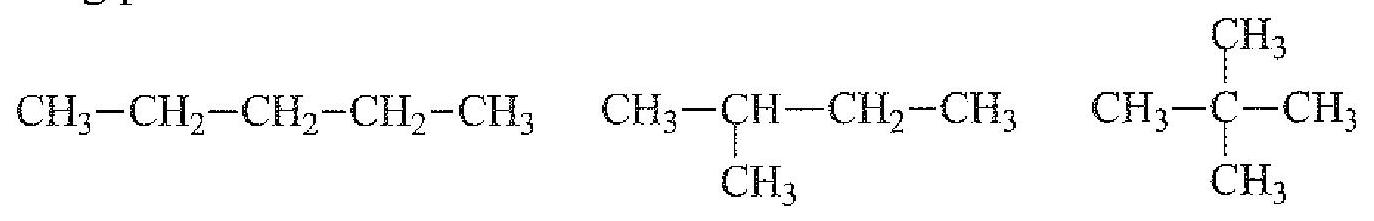
\includegraphics[max width=\textwidth, center]{2025_10_23_ed7118e3280f74e91193g-21(1)}\\
$\mathrm{C}_{4} \mathrm{H}_{8}$ có các đồng phân cấu tạo về mạch carbon và vị trí liên kết $\pi$ của hydrocarbon chưa no, mạch hở, phân tử có một liên kết đôi và đồng phân về mạch carbon của hydrocarbon no, mạch vòng.\\
Các đồng phân:

$$
\begin{aligned}
& \mathrm{CH}_{2}=\mathrm{CH}-\mathrm{CH}_{2}-\mathrm{CH}_{3} \\
& \mathrm{CH}_{3}-\mathrm{CH}=\mathrm{CH}-\mathrm{CH}_{3} \\
& \mathrm{CH}_{2}=\mathrm{C}_{\mathrm{CH}}-\mathrm{CH}_{3} \\
& \mathrm{CH}_{3}
\end{aligned}
$$

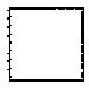
\includegraphics[max width=\textwidth, center]{2025_10_23_ed7118e3280f74e91193g-21}\\
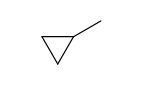
\includegraphics{smile-46a9fecad658203382dd7bf14930aef48e7c6a34}\\
13.12. $\mathrm{C}_{4} \mathrm{H}_{10} \mathrm{O}$ có các đồng phân về loại nhóm chức (alcohol và ether), mạch carbon và vị trí nhóm chức.\\
Các đồng phân:\\
$\mathrm{CH}_{3}-\mathrm{CH}_{2}-\mathrm{CH}_{2}-\mathrm{CH}_{2}-\mathrm{OH}$\\
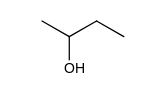
\includegraphics{smile-e3cd5a943d2077ded51796bb95b17b0be837e8b2}\\
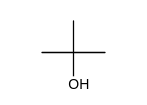
\includegraphics{smile-c6a305275eec148796f60ddf4d287a92f1ef034a}\\
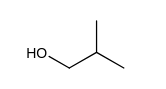
\includegraphics{smile-0f8d6d57c76317aa72a062030d1d18d40daf14a9}\\
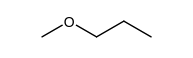
\includegraphics{smile-09ac599a594901e1eb1ad5572fdf6614c9881444}\\
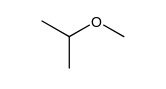
\includegraphics{smile-3d85f430c8220dd35c3f0d0c56bc240f0efa0217}

$$
\mathrm{CH}_{3}-\mathrm{CH}_{2}-\mathrm{O}-\mathrm{CH}_{2}-\mathrm{CH}_{3}
$$

\section*{EAI 14. ÔN TÂP CHUONG 3}
\begin{center}
\begin{tabular}{|c|c|c|c|}
\hline
$14.1 . \mathrm{A}$ & $14.2 . \mathrm{B}$ & $14.3 . \mathrm{B}$ & $14.4 . \mathrm{C}$ \\
\hline
$14.5 . \mathrm{D}$ & $14.6 . \mathrm{D}$ & $14.7 . \mathrm{B}$ & $14.8 . \mathrm{C}$ \\
\hline
\end{tabular}
\end{center}

14.6. Ethanol được tách bằng phương pháp chưng cất.\\
14.9. Butane thuộc loại alkane, but-1-ene thuộc loại alkene và but-2-yne thuộc loại alkyne.\\
14.10. Công thức tổng quát của Atabrine có dạng $\mathrm{C}_{\mathrm{x}} \mathrm{H}_{\mathrm{y}} \mathrm{O}_{\mathrm{z}} \mathrm{N}_{\mathrm{t}} \mathrm{Cl}_{\mathrm{u}}$.

Ta có: $\mathrm{x}: \mathrm{y}: \mathrm{z}: \mathrm{t}: \mathrm{u}=\frac{69,1}{12}: \frac{7,5}{1}: \frac{4,0}{16}: \frac{10,5}{14}: \frac{8,9}{35,5}$

$$
=5,76: 7,50: 0,25: 0,75: 0,25=23: 30: 1: 3: 1 .
$$

$\Rightarrow$ Công thức thực nghiệm của Atabrine là $\mathrm{C}_{23} \mathrm{H}_{30} \mathrm{ON}_{3} \mathrm{Cl}$.\\
14.11. Công thức tổng quát của Aspirin là $\mathrm{C}_{\mathrm{x}} \mathrm{H}_{\mathrm{y}} \mathrm{O}_{\mathrm{z}}$.

Phân tử khối theo phổ khối lượng là 180.\\
Ta có : $\frac{12 x}{60,00}=\frac{y}{4,44}=\frac{16 z}{35,56}=\frac{180}{100}$.\\
$\Rightarrow x=9, y=8, z=4 \Rightarrow$ công thức phân tử của Aspirin là $\mathrm{C}_{9} \mathrm{H}_{8} \mathrm{O}_{4}$.\\
14.12. $\mathrm{C}_{4} \mathrm{H}_{9} \mathrm{Cl}$ có đồng phân cấu tạo về mạch carbon và vị trí nhóm thế (nhóm -Cl ) trên mạch.

$$
\mathrm{CH}_{3}-\mathrm{CH}_{2}-\mathrm{CH}_{2}-\mathrm{CH}_{2}-\mathrm{Cl}
$$

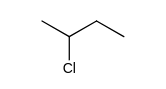
\includegraphics{smile-2ec7ac6dfb6e62c0b03300233410ccf59d7e1556}\\
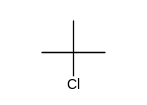
\includegraphics{smile-ec4a74aaf271388cffb4d7f8b6e6f4c4e087294c}\\
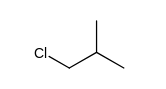
\includegraphics{smile-1b584556796801f1626d1acbe0676d9eb09fbff7}\\
$\mathrm{C}_{8} \mathrm{H}_{10}$ (hydrocarbon thơm) có đồng phân về vị trí tương đối của các nhóm thế trên vòng benzene.\\
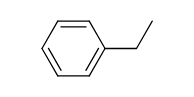
\includegraphics{smile-123878df13b8c2072625659d1b6e1325791b2812}\\
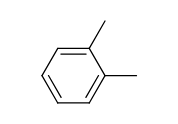
\includegraphics{smile-8fe4f93d6fbd7a20f3cb0893f5be7876b3a23e79}\\
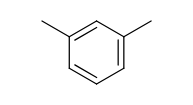
\includegraphics{smile-ab9cc2604bb68fce806bfa076053e5f7e9c2476d}\\
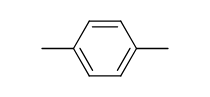
\includegraphics{smile-3c58c693532a408942972be111f496131deb08ab}

\section*{Ch110110. \\
 INOROCARBON}
\section*{DAII 5. \\
 ALKANE}
\begin{center}
\begin{tabular}{|l|l|l|l|l|l|}
\hline
$15.1 . \mathrm{B}$ & $15.2 . \mathrm{B}$ & $15.3 . \mathrm{A}$ & $15.4 . \mathrm{D}$ & $15.5 . \mathrm{D}$ & $15.6 . \mathrm{A}$ \\
\hline
$15.7 . \mathrm{D}$ & $15.8 . \mathrm{C}$ & $15.9 . \mathrm{A}$ & $15.10 . \mathrm{D}$ & $15.11 . \mathrm{D}$ & $15.12 . \mathrm{D}$ \\
\hline
$15.13 . \mathrm{A}$ & $15.14 . \mathrm{B}$ & $15.15 . \mathrm{B}$ & $15.16 . \mathrm{A}$ & $15.17 . \mathrm{D}$ & $15.18 . \mathrm{B}$ \\
\hline
\end{tabular}
\end{center}

15.4. D sai: Trong phân tử methane, bốn liên kết $\mathrm{C}-\mathrm{H}$ giống nhau tạo với thau một góc $109,5^{\circ}$ và hướng về bốn đỉnh của một tứ diện đều.\\
15.12. 5 đồng phân gồm:\\
$\mathrm{CH}_{3}\left[\mathrm{CH}_{2}\right]_{4} \mathrm{CH}_{3} ; \mathrm{CH}_{3} \mathrm{CH}\left(\mathrm{CH}_{3}\right) \mathrm{CH}_{2} \mathrm{CH}_{2} \mathrm{CH}_{3} ; \mathrm{CH}_{3} \mathrm{CH}_{2} \mathrm{CH}\left(\mathrm{CH}_{3}\right) \mathrm{CH}_{2} \mathrm{CH}_{3} ;$\\
$\mathrm{CH}_{3} \mathrm{CH}\left(\mathrm{CH}_{3}\right) \mathrm{CH}\left(\mathrm{CH}_{3}\right) \mathrm{CH}_{3} ;\left(\mathrm{CH}_{3}\right)_{3} \mathrm{CCH}_{2} \mathrm{CH}_{3}$.\\
15.16. Thu được sản phẩm duy nhất là 1-chloro-2,2-dimethylpropane.\\
15.17. Reforming alkane là quá trình chuyển các alkane mạch không phân nhánh thành các alkane mạch phân nhánh và các hydrocarbon mạch vòng nhưng không làm thay đổi số nguyên tử carbon trong phân tử.\\
15.19. a) Công thức cấu tạo:\\
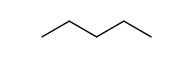
\includegraphics{smile-72adf3ca2775db4852c7dc2055d55c10ac742ee1}

pentane\\
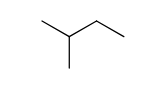
\includegraphics{smile-8d344d449d9937686169dea673073c9d5488b778}\\
isopentane\\
2-methylbutane\\
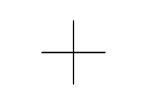
\includegraphics{smile-97b5d12e87770889267767a0401ba276a36f3d65}\\
neopentane\\
2,2-dimethylpropane\\
b) Tên goi các alkane:

(i)\\
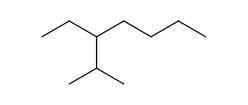
\includegraphics{smile-96d47cbf41c264311a8cee82b56cd0ad84646f9c}

3-ethyl-2-methylheptane

(ii)\\
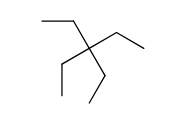
\includegraphics{smile-13a4f1e9f8f6f77e005c0033b736234a9ddcd9aa}

3,3-diethylpentane\\
15.20. a) Hai sản phẩm:\\
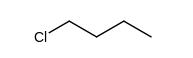
\includegraphics{smile-fa8f3c6d0bd90a5e1d39b2fc80aa4f8ff132068c}

1-chlorobutane\\
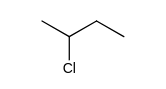
\includegraphics{smile-762bef93410011c817917fee1eb90b9e01eb4de1}

2-chlorobutane\\
b) Hai săn phẩm:\\
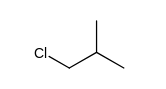
\includegraphics{smile-7ea2cab81c1d2fa898c0047d47a0ee69e4ae639f}

1-chloro-2-methylpropane\\
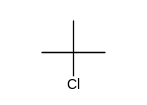
\includegraphics{smile-1e00284413d7d159ebb51408273bf164216386bb}

2-chloro-2-methylpropane\\
c) Một sản phẩm:\\
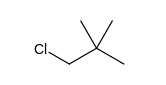
\includegraphics{smile-9359858e24c4974c03e3b9544063860ed11b9388}

1-chloro-2,2-dimethylpropane\\
15.21. a) Bậc của carbon càng cao, phản ứng thế xảy ra càng dễ dàng. Phản ứng thế ở carbon bậc ba dễ hơn ở carbon bậc hai và phản ứng thế ở carbon bậc hai dễ hơn ở carbon bậc một.\\
b) Chlorine tham gia phản ưng thế dễ dàng hơn so với bromine. Vi vậy, tính chọn lọc vị trí thế của chlorine yếu hơn so với bromine (nói cách khác, do khả năng phản ứng của bromine yếu, nên bromine chủ yếu lựa chọn phản ứng ở vị trí carbon bậc cao hon, nơi phản ứng xảy ra dễ dàng hơn).\\
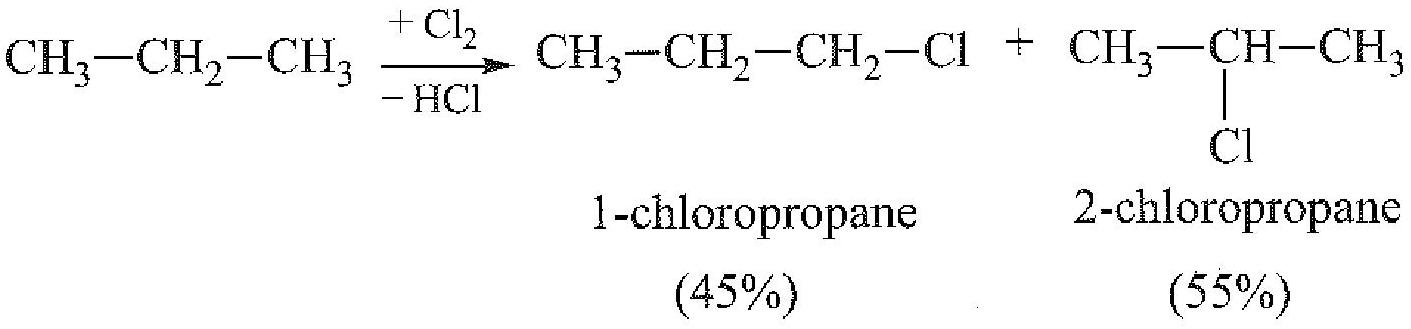
\includegraphics[max width=\textwidth, center]{2025_10_23_ed7118e3280f74e91193g-24}\\
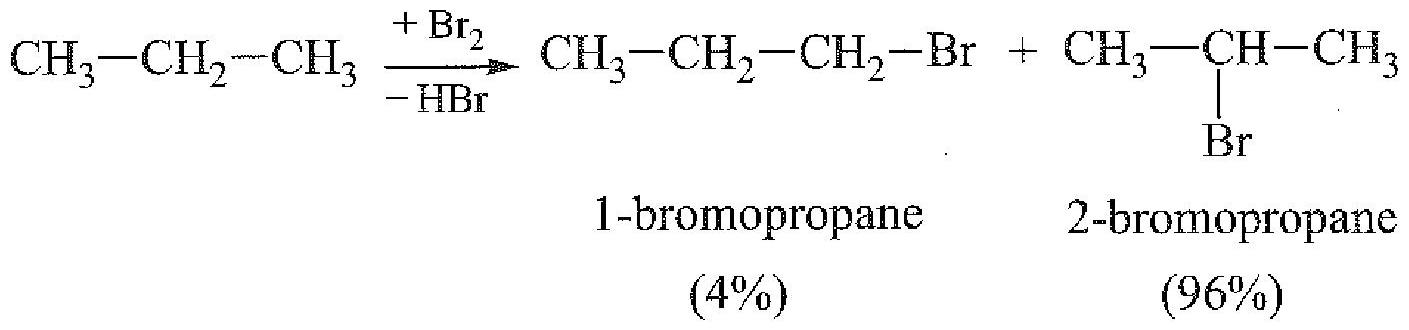
\includegraphics[max width=\textwidth, center]{2025_10_23_ed7118e3280f74e91193g-24(1)}\\
15.22. Nhiệt cháy của methane là biến thiên enthalpy của phản ứng:\\
$\mathrm{CH}_{4}(\mathrm{~g})+2 \mathrm{O}_{2}(\mathrm{~g}) \longrightarrow \mathrm{CO}_{2}(\mathrm{~g})+2 \mathrm{H}_{2} \mathrm{O}(l)$\\
$\Delta \mathrm{H}_{\text {đót cháy } \mathrm{CH}_{4}}^{\mathrm{o}}=1 \cdot \Delta_{\mathrm{f}} \mathrm{H}_{\mathrm{CO}_{2}}^{\mathrm{o}}+2 \cdot \Delta_{\mathrm{f}} \mathrm{H}_{\mathrm{H}_{2} \mathrm{O}}^{\mathrm{o}}-1 \cdot \Delta_{\mathrm{f}} \mathrm{H}_{\mathrm{CH}_{4}}^{\mathrm{o}}-2 \cdot \Delta_{\mathrm{f}} \mathrm{H}_{\mathrm{O}_{2}}^{\mathrm{o}}$.\\
Vậy nhiệt hình thành chuẩn của methane là:\\
$\Delta_{\mathrm{f}} \mathrm{H}_{\mathrm{CH}_{4}}^{\mathrm{o}}=1 \cdot(-393,5)+2 \cdot(-285,8)-1 \cdot(-890)=-75,1(\mathrm{~kJ} / \mathrm{mol})$.\\
Nhiệt cháy của propane là biến thiên enthalpy của phản ứng:\\
$\mathrm{C}_{3} \mathrm{H}_{8}(\mathrm{~g})+5 \mathrm{O}_{2}(\mathrm{~g}) \longrightarrow 3 \mathrm{CO}_{2}(\mathrm{~g})+4 \mathrm{H}_{2} \mathrm{O}(\mathrm{l})$\\
$\Delta \mathrm{H}_{\text {dót cháy } \mathrm{C}_{3} \mathrm{H}_{8}}^{\mathrm{o}}=3 \cdot \Delta_{\mathrm{f}} \mathrm{H}_{\mathrm{CO}_{2}}^{\mathrm{o}}+4 \cdot \Delta_{\mathrm{f}} \mathrm{H}_{\mathrm{H}_{2} \mathrm{O}}^{\mathrm{o}}-1 \cdot \Delta_{\mathrm{f}} \mathrm{H}_{\mathrm{C}_{3} \mathrm{H}_{8}}^{\mathrm{o}}-5 \cdot \Delta_{\mathrm{f}} \mathrm{H}_{\mathrm{O}_{2}}^{\mathrm{o}}$.\\
Vậy nhiệt hìrh thành chuẩn của propane là:\\
$\Delta_{\mathrm{f}} \mathrm{H}_{\mathrm{C}_{3} \mathrm{H}_{8}}^{\mathrm{o}}=3 \cdot(-393,5)+4 \cdot(-285,8)-1 \cdot(-2216)=-107,7(\mathrm{~kJ} / \mathrm{mol})$.

\section*{BAI 16. HYDROCARBON KHÔNG NO}
\begin{center}
\begin{tabular}{|c|c|c|c|c|}
\hline
$16.1 . \mathrm{C}$ & $16.2 . \mathrm{B}$ & $16.3 . \mathrm{C}$ & $16.4 . \mathrm{A}$ & $16.5 . \mathrm{B}$ \\
\hline
$16.6 . \mathrm{B}$ & $16.7 . \mathrm{D}$ & $16.8 . \mathrm{D}$ & $16.9 . \mathrm{A}$ & $16.10 . \mathrm{C}$ \\
\hline
$16.11 . \mathrm{C}$ & $16.12 . \mathrm{B}$ & $16.13 . \mathrm{D}$ & $16.14 . \mathrm{C}$ &  \\
\hline
\end{tabular}
\end{center}

16.9. Các đồng phân:\\
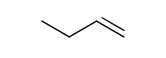
\includegraphics{smile-d1989dba5b137c6f5b8579b645fa485fe0c799f6}

but-1-ene\\
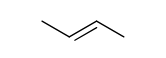
\includegraphics{smile-7f2337270553a145e384a8290ceaa72d5827c4f6}

trans-but-2-ene\\
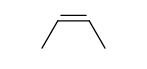
\includegraphics{smile-4e3263dbe0063fb7011f0228b289f87a9daf5db8}

cis-but-2-ene\\
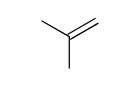
\includegraphics{smile-00f22c15b39587d8094e7b844147abd44453175a}

2-methylprop-1-ene\\
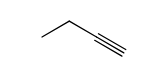
\includegraphics{smile-1bd32dcee57ebfeda3ee19fa8564eec9a57c3b15}

but-1-yne

\begin{figure}[h]
\begin{center}
  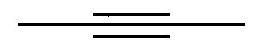
\includegraphics[width=\textwidth]{2025_10_23_ed7118e3280f74e91193g-25}
\captionsetup{labelformat=empty}
\caption{but-2-yne}
\end{center}
\end{figure}

16.14. Các alkyne có liên kết ba ở đầu mạch (alk-1-yne) có khả năng tham gia phản ứng với dung dịch $\mathrm{AgNO}_{3}$ trong $\mathrm{NH}_{3}$ tạo thành kết tủa.\\
16.15. Các sản phẩm chính và tên gọi:\\
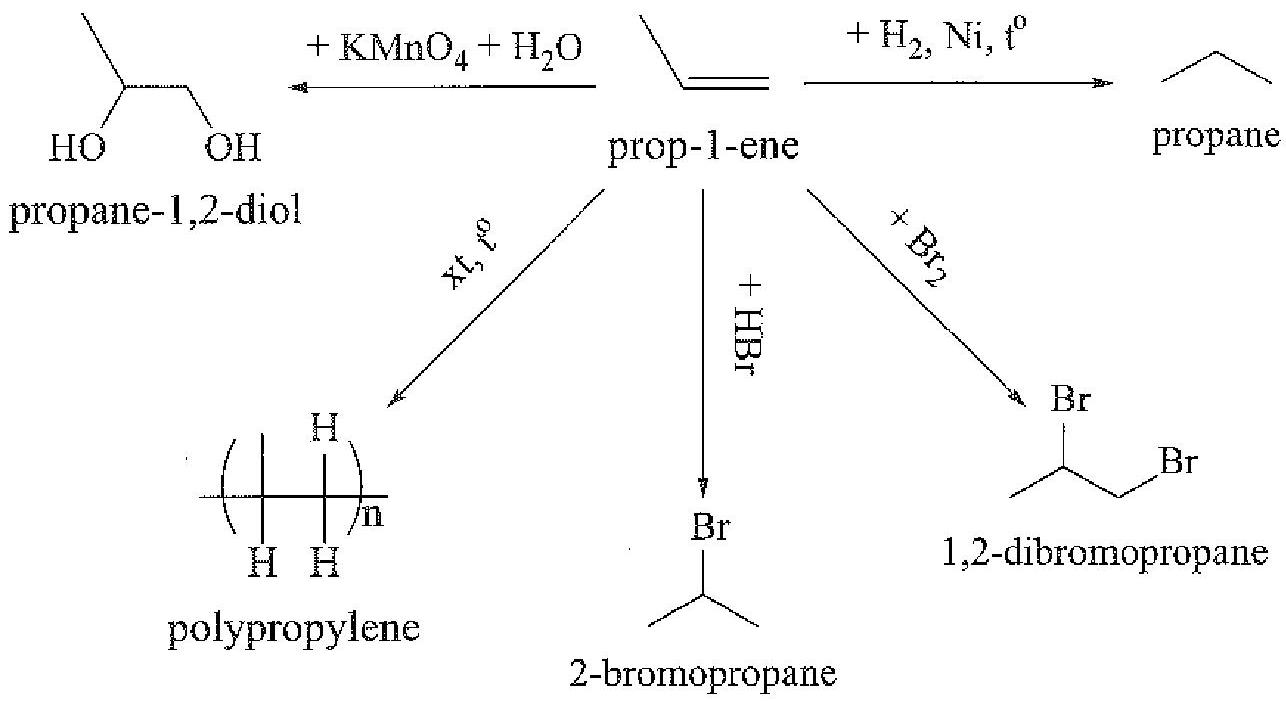
\includegraphics[max width=\textwidth, center]{2025_10_23_ed7118e3280f74e91193g-26(1)}\\
16.16. Các sản phẩm chính và tên gọi:\\
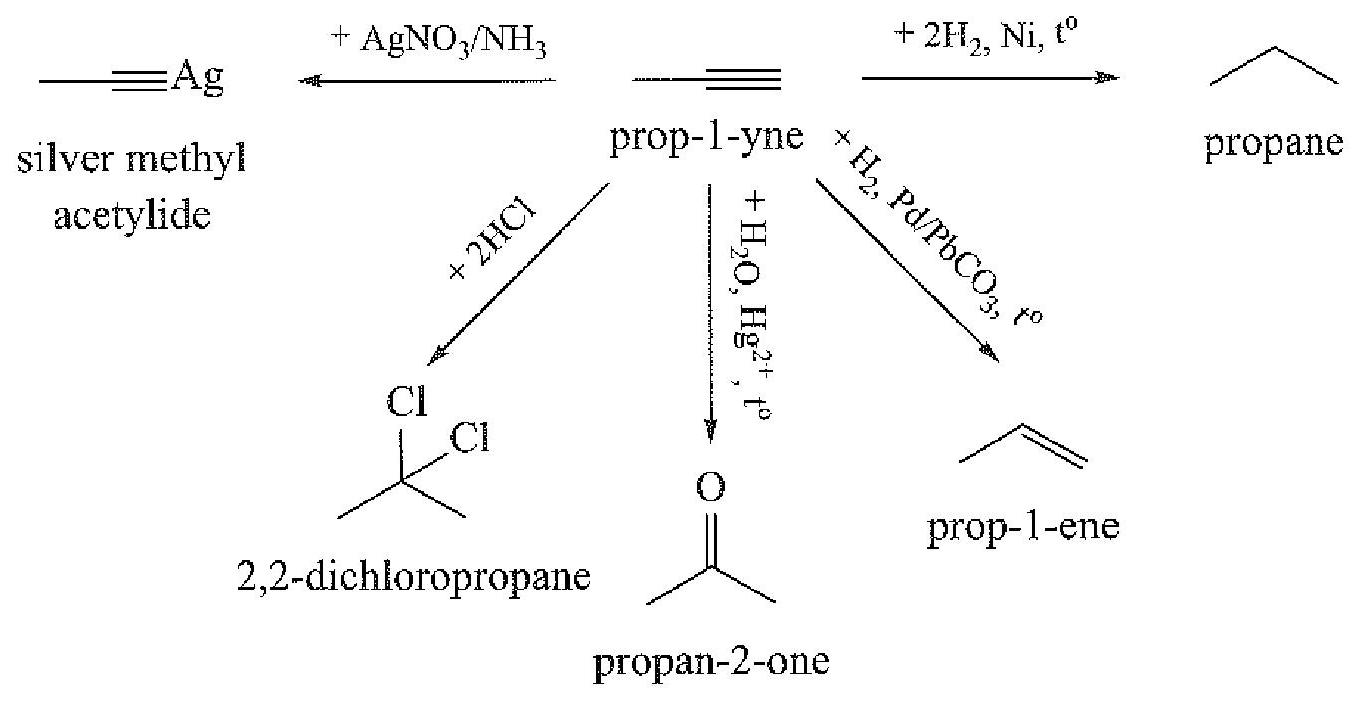
\includegraphics[max width=\textwidth, center]{2025_10_23_ed7118e3280f74e91193g-26}\\
16.17. A là acetylene, B là ethylene, C là 1,2 -dichloroethane và D là chloroethene (vinyl chloride)\\
$2 \mathrm{CH}_{4}+\frac{3}{2} \mathrm{O}_{2} \xrightarrow{\mathrm{xt}_{, \mathrm{t}^{\mathrm{o}}}} \mathrm{CH} \equiv \mathrm{CH}+3 \mathrm{H}_{2} \mathrm{O}$\\
$\mathrm{CH} \equiv \mathrm{CH}+\mathrm{HCl} \xrightarrow{\mathrm{HgCl}_{2}, \mathrm{t}^{\circ}} \mathrm{CH}_{2}=\mathrm{CHCl}$\\
$\mathrm{CH} \equiv \mathrm{CH}+\mathrm{H}_{2} \xrightarrow{\mathrm{Pd} / \mathrm{PbCO}_{3}, \mathrm{t}^{\circ}} \mathrm{CH}_{2}=\mathrm{CH}_{2}$\\
$\mathrm{CH}_{2}=\mathrm{CH}_{2}+\mathrm{Cl}_{2} \longrightarrow \mathrm{CH}_{2} \mathrm{Cl}-\mathrm{CH}_{2} \mathrm{Cl}$\\
$\mathrm{CH}_{2} \mathrm{Cl}-\mathrm{CH}_{2} \mathrm{Cl} \xrightarrow{377^{\circ} \mathrm{C}} \mathrm{CH}_{2}=\mathrm{CHCl}+\mathrm{HCl}$\\
$\mathrm{nCH}_{2}=\mathrm{CHCl} \xrightarrow{\mathrm{xt}^{\mathrm{e}} \mathrm{t}^{\circ}}-\left(\mathrm{CH}_{2}-\mathrm{CHCl}\right)_{\mathrm{n}}$

\section*{BAI17.}
\section*{AREN (HYDROCARBON THOM)}
\begin{center}
\begin{tabular}{|c|c|c|c|c|}
\hline
17.1. A & 17.2. D & 17.3. C & 17.4. D & 17.5. C \\
\hline
17.6. D & 17.7. D & 17.8. D & 17.9. D & 17.10. C \\
\hline
17.11. A & 17.12. C & 17.13. A & 17.14. C &  \\
\hline
\end{tabular}
\end{center}

17.5. Khi benzene có nhóm thế alkyl ( $-\mathrm{CH}_{3},-\mathrm{C}_{2} \mathrm{H}_{5}, \ldots$ ), các phản úng thế nguyên tử hydrogen ở vòng benzene xảy ra dễ dàng hơn so với benzene và ưu tiên thể vào vị trí số 2 hoặc số 4 (vị trí ortho hoặc para) so với nhóm alkyl.\\
17.15. Các đồng phân và tên gọi:\\
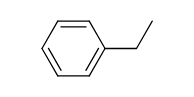
\includegraphics{smile-7b20fa2c6094ebc9edaac2291b6dd9a41d95271f}

ethylbenzene\\
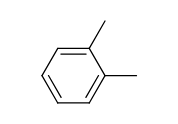
\includegraphics{smile-ada42d2954463b021724bfce25bf6f15ae852efd}

o-xylene\\
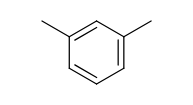
\includegraphics{smile-907fc6a2d8a44cd774d6e7ad1f4231b9b516bfab}

m-xylene\\
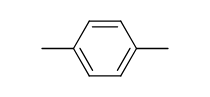
\includegraphics{smile-67610e9fb0b45057c2e3bce5b082eadec82d42d4}

$p$-xylene\\
17.16. Chất X là nitrobenzene

$$
\mathrm{C}_{6} \mathrm{H}_{6}+\mathrm{HONO}_{2} \xrightarrow{\mathrm{H}_{2} \mathrm{SO}_{4} \text { đặc }} \mathrm{C}_{6} \mathrm{H}_{5} \mathrm{NO}_{2}+\mathrm{H}_{2} \mathrm{O}
$$

17.17. Các sản phẩm chính và tên gọi:\\
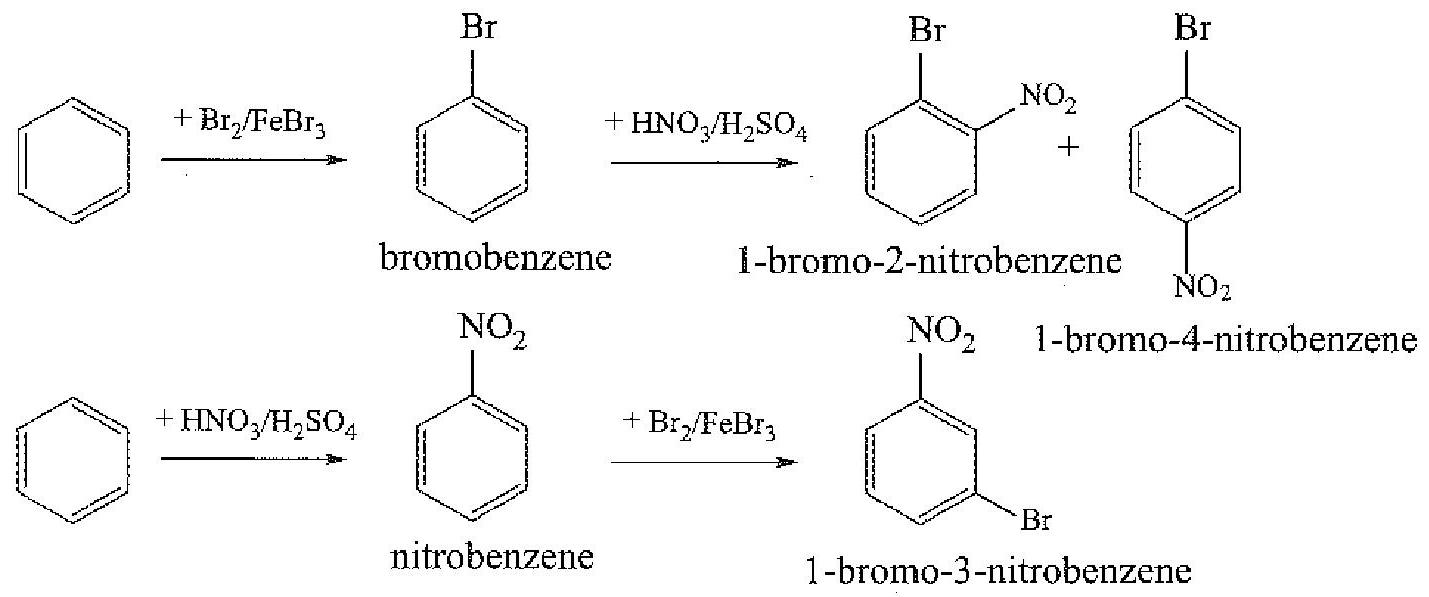
\includegraphics[max width=\textwidth, center]{2025_10_23_ed7118e3280f74e91193g-27}\\
17.18. Các sản phẩm chính và tên goit:\\
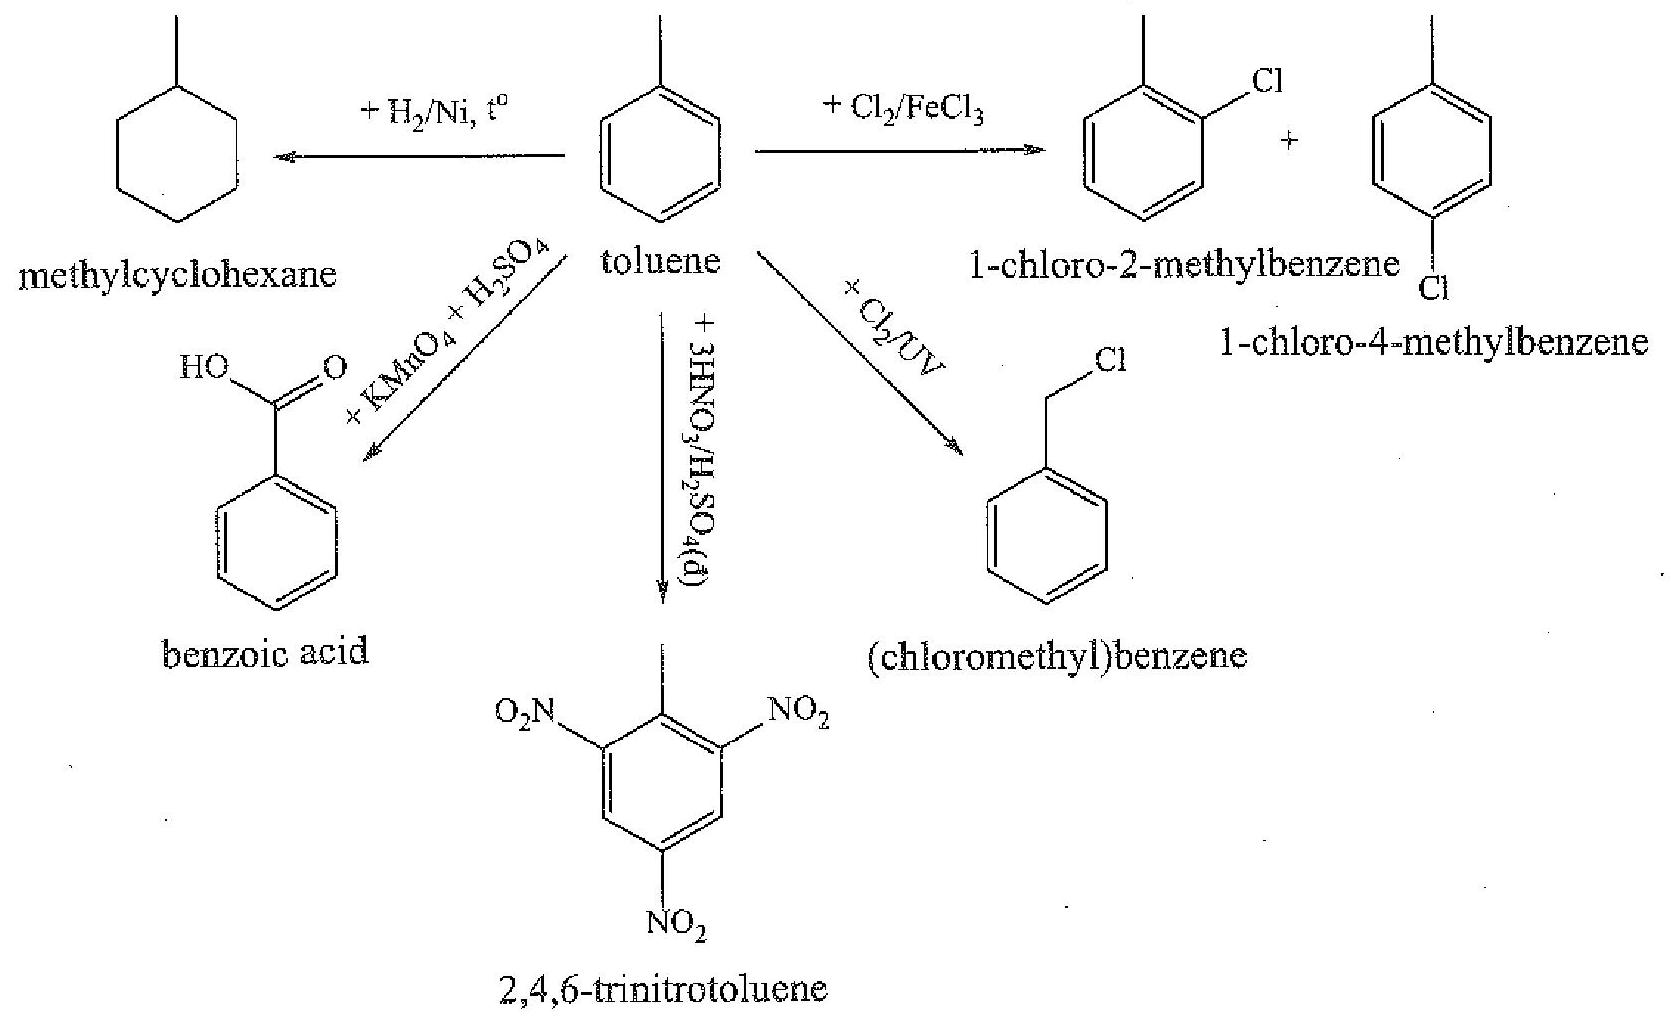
\includegraphics[max width=\textwidth, center]{2025_10_23_ed7118e3280f74e91193g-28}\\
17.19. a) Điều chế polystyrene từ hexane:\\
$\mathrm{C}_{6} \mathrm{H}_{14} \xrightarrow{\text { reforming }} \mathrm{C}_{6} \mathrm{H}_{6}+4 \mathrm{H}_{2}$\\
$\mathrm{C}_{6} \mathrm{H}_{6}+\mathrm{CH}_{2}=\mathrm{CH}_{2} \xrightarrow{\mathrm{H}^{+}} \mathrm{C}_{6} \mathrm{H}_{5} \mathrm{CH}_{2} \mathrm{CH}_{3}$\\
$\mathrm{C}_{6} \mathrm{H}_{5} \mathrm{CH}_{2} \mathrm{CH}_{3} \xrightarrow{\mathrm{xt}, \mathrm{t}^{\circ}} \mathrm{C}_{6} \mathrm{H}_{5} \mathrm{CH}=\mathrm{CH}_{2}+\mathrm{H}_{2}$\\
$\mathrm{C}_{6} \mathrm{H}_{5} \mathrm{CH}=\mathrm{CH}_{2} \xrightarrow{\mathrm{xt}_{2} \mathrm{t}^{\mathrm{e}}}+\left(\mathrm{CH}\left(\mathrm{C}_{6} \mathrm{H}_{5}\right)-\mathrm{CH}_{2}\right)_{n}$\\
b) 2,4,6-trinitrotoluene từ heptane:\\
$\mathrm{C}_{7} \mathrm{H}_{16} \xrightarrow{\text { reforming }} \mathrm{C}_{6} \mathrm{H}_{5} \mathrm{CH}_{3}+4 \mathrm{H}_{2}$\\
$\mathrm{C}_{6} \mathrm{H}_{5} \mathrm{CH}_{3}+3 \mathrm{HONO}_{2} \xrightarrow{\mathrm{H}_{2} \mathrm{SO}_{4} \text { đăc }} 2,4,6-\left(\mathrm{O}_{2} \mathrm{~N}\right)_{3} \mathrm{C}_{6} \mathrm{H}_{2} \mathrm{CH}_{3}+3 \mathrm{H}_{2} \mathrm{O}$

\section*{BAL 18. ÔN TÂP CHUONG 4}
\begin{center}
\begin{tabular}{|c|c|c|c|c|}
\hline
$18.1 . \mathrm{D}$ & $18.2 . \mathrm{D}$ & $18.3 . \mathrm{A}$ & $18.4 . \mathrm{B}$ & $18.5 . \mathrm{D}$ \\
\hline
$18.6 . \mathrm{B}$ & $18.7 . \mathrm{C}$ & $18.8 . \mathrm{B}$ & $18.9 . \mathrm{A}$ &  \\
\hline
\end{tabular}
\end{center}

18.10. a) Ethane, ethylene, acetylene và butane là những chất khí; benzene và styrene là những chất lỏng; naphtalene là chất rắn.\\
b) Phân tử các hydrocarbon không phân cực hoặc kém phân cực, nên không tan hoặc it tan trong nước (là một dung môi phân cực), nhưng tan nhiều trong các dung môi hữu cơ (là những dung môi phân cực kém (hay it phân cực)).\\
18.11. - Alkane 5C:\\
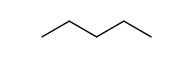
\includegraphics{smile-2ccee4c44810ebbef84f1a2e90135be482aca89b}

pentane\\
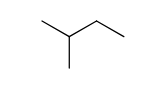
\includegraphics{smile-c5590549eecd6142e008f1d09b9644bf1f1b423f}

isopentane\\
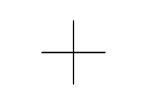
\includegraphics{smile-aa44cf304737f87d7eed2ebd03183d4ffa21f075}

neopentane

\begin{itemize}
  \item Alkene 5C:\\
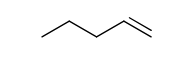
\includegraphics{smile-d4cbd49d128915922ac6eeb2b3eee303e2e8448c}
\end{itemize}

pent-1-ene\\
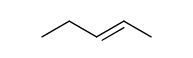
\includegraphics{smile-fb05e63fafd14643155c4e815f3857d2c0211381}

trans-pent-2-ene\\
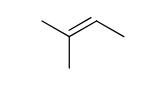
\includegraphics{smile-08058f48ee85152196c907e44768c7ea10784b6f}

2-methylbut-2-ene\\
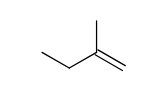
\includegraphics{smile-1f20a45801cc60f31affcb92093831d0deb8ab46}

2-methylbut-1-ene\\
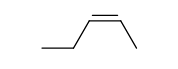
\includegraphics{smile-e63164adf66508c18c67321e7d13df249fd4156a}

cis-pent-2-ene\\
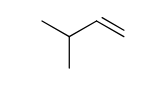
\includegraphics{smile-52cdad411f730e00ab18ae851a1ba552d8df1c3b}

3-methylbut-1-ene

\begin{itemize}
  \item Alkyne 5C:\\
\includegraphics{smile-dd8457a7758b932a36c768d082994d70c31d7f6b}
\end{itemize}

pent-1-yne\\
\includegraphics{smile-68f841a60f7fa96a58870a6949b534cac7ac2bd5}

pent-2-yne\\
\includegraphics{smile-aec80ec7eaa908d3348e0d40f644907da106a496}

3-methylbut-1-yne

\begin{itemize}
  \item Đồng đẳng của benzene 8 C :\\
\includegraphics{smile-138c8f8dffe228bece51de15f6355cf29679262b}
\end{itemize}

ethylbenzene\\
\includegraphics{smile-27855cb0823ad2fc00deef508e38e81b7ec590c2}

o-xylene\\
\includegraphics{smile-8945d422a11b2019efcb836d4bb5b84efc050702}

$m$-xylene\\
\includegraphics{smile-40ef967be8f437b4697577099576d2725532412d}

$p$-xylene\\
18.12. Các phương trình hoá học:\\
(1) $\mathrm{CH}_{4}+\mathrm{Cl}_{2} \xrightarrow{\text { ánh sáng }} \mathrm{CH}_{3} \mathrm{Cl}+\mathrm{HCl}$\\
(2) $\mathrm{CH}_{4}+\frac{3}{2} \mathrm{O}_{2} \xrightarrow{\mathrm{t}^{\circ}} \mathrm{CO}_{2}+\mathrm{H}_{2} \mathrm{O}$\\
(3) $2 \mathrm{CH}_{4} \xrightarrow{\mathrm{xt}, \mathrm{t}^{\mathrm{o}}} \mathrm{CH} \equiv \mathrm{CH}+3 \mathrm{H}_{2}$\\
(4) $\mathrm{CH} \equiv \mathrm{CH}+\mathrm{HCl} \xrightarrow{\mathrm{Hg}^{2+}, \mathrm{t}^{\circ}} \mathrm{CH}_{2}=\mathrm{CHCl}$\\
(5) $\mathrm{CH}=\mathrm{CH}+\mathrm{H}_{2} \mathrm{O} \xrightarrow{\mathrm{Hg}^{2+}, \mathrm{t}^{\circ}} \mathrm{CH}_{3} \mathrm{CH}=\mathrm{O}$\\
(6) $\mathrm{CH} \equiv \mathrm{CH}+\mathrm{H}_{2} \xrightarrow{\mathrm{Pd} / \mathrm{PbCO}_{3}, \mathrm{t}^{\circ}} \mathrm{CH}_{2}=\mathrm{CH}_{2}$\\
(7) $\mathrm{CH}_{2}=\mathrm{CH}_{2}+\mathrm{H}_{2} \mathrm{O} \xrightarrow{\mathrm{H}^{+}, \mathrm{t}^{\mathrm{a}}} \mathrm{CH}_{3} \mathrm{CH}_{2} \mathrm{OH}$\\
(8) $3 \mathrm{CH}_{2}=\mathrm{CH}_{2}+2 \mathrm{KMnO}_{4}+4 \mathrm{H}_{2} \mathrm{O} \longrightarrow 3 \mathrm{CH}_{2}(\mathrm{OH}) \mathrm{CH}_{2}(\mathrm{OH})+2 \mathrm{MnO}_{2}+2 \mathrm{KOH}$\\
(9) $\mathrm{nCH}_{2}=\mathrm{CH}_{2} \xrightarrow{\mathrm{xt}, \mathrm{t}^{\mathrm{o}}}+\mathrm{CH}_{2}-\mathrm{CH}_{2}$ ) $\frac{\pi}{\pi}$\\
18.13. Các phương trình hoá học:\\
(1) $\mathrm{CH}_{3}\left[\mathrm{CH}_{2}\right]_{4} \mathrm{CH}_{3} \xrightarrow{\text { cracking }} \mathrm{CH}_{3} \mathrm{CH}_{2} \mathrm{CH}_{3}+\mathrm{CH}_{3} \mathrm{CH}=\mathrm{CH}_{2}$\\
(2) $\mathrm{CH}_{3} \mathrm{CH}_{2} \mathrm{CH}_{3}+\mathrm{Cl}_{2} \xrightarrow{\text { ánh sáng }} \mathrm{CH}_{3} \mathrm{CHClCH}_{3}+\mathrm{HCl}$\\
(3) $\mathrm{CH}_{3}\left[\mathrm{CH}_{2}\right]_{4} \mathrm{CH}_{3} \xrightarrow{\text { cracking }} \mathrm{CH}_{3} \mathrm{CH}_{3}+\mathrm{CH}_{3} \mathrm{CH}_{2} \mathrm{CH}=\mathrm{CH}_{2}$\\
(4) $\mathrm{CH}_{3} \mathrm{CH}_{2} \mathrm{CH}=\mathrm{CH}_{2}+\mathrm{HCl} \longrightarrow \mathrm{CH}_{3} \mathrm{CH}_{2} \mathrm{CHClCH}_{3}$\\
(5) $\mathrm{CH}_{3}\left[\mathrm{CH}_{2}\right]_{4} \mathrm{CH}_{3} \xrightarrow{\text { reforming }} \mathrm{C}_{6} \mathrm{H}_{6}+4 \mathrm{H}_{2}$\\
(6) $\mathrm{C}_{6} \mathrm{H}_{6}+2 \mathrm{Cl}_{2} \xrightarrow{\mathrm{Fe}, \mathrm{t}^{\circ}} o-\mathrm{C}_{6} \mathrm{H}_{4}\left(\mathrm{Cl}_{2}\right.$ và $p-\mathrm{C}_{6} \mathrm{H}_{4}\left(\mathrm{Cl}_{2}+2 \mathrm{HCl}\right.$\\
(7) $\mathrm{C}_{6} \mathrm{H}_{6}+2 \mathrm{HNO}_{3} \xrightarrow{\mathrm{H}_{2} \mathrm{SO}_{4}, \mathrm{t}^{\circ}} \mathrm{m}-\mathrm{C}_{6} \mathrm{H}_{4}\left(\mathrm{NO}_{2}\right)_{2}+2 \mathrm{H}_{2} \mathrm{O}$

\section*{Churong 5 DAN XUAT IALOGEN ALCOHOL-PHENOL}
\section*{BAlle. DÃN XUÁT HALOGEN}
\begin{center}
\begin{tabular}{|c|c|c|c|c|}
\hline
$19.1 . \mathrm{D}$ & $19.2 . \mathrm{B}$ & $19.3 . \mathrm{C}$ & $19.4 . \mathrm{C}$ & $19.5 . \mathrm{A}$ \\
\hline
$19.6 . \mathrm{B}$ & $19.7 . \mathrm{C}$ & $19.8 . \mathrm{B}$ & $19.9 . \mathrm{D}$ & $19.10 . \mathrm{A}$ \\
\hline
\end{tabular}
\end{center}

19.11. Dẫn xuất halogen bị thế nguyên tử halogen:\\
$\mathrm{CH}_{2}=\mathrm{CHCH}_{2} \mathrm{Br}+\mathrm{NaOH} \xrightarrow{\mathrm{t}^{\circ}} \mathrm{CH}_{2}=\mathrm{CHCH}_{2} \mathrm{OH}+\mathrm{NaBr}$\\
Trung hoà bằng đung dịch $\mathrm{HNO}_{3}$ để loại bỏ kiềm dư.\\
Nhỏ dung dịch $\mathrm{AgNO}_{3}$ vào ống nghiệm, xuất hiện kết tủa vàng nhạt:\\
$\mathrm{AgNO}_{3}+\mathrm{NaBr} \longrightarrow \mathrm{AgBr}+\mathrm{NaNO}_{3}$.\\
19.12. Công thức cấu tạo các dẫn xuất halogen có trong R-45B:

Difluoromethane: $\mathrm{CH}_{2} \mathrm{~F}_{2} ; 2,3,3,3$-tetrafluoropropene: $\mathrm{CH}_{2} \mathrm{CFCF}_{3}$.\\
19.13. a) $\mathrm{C}_{4} \mathrm{H}_{9} \mathrm{Br}$ có 4 dồng phân cấu tạo sau:\\
$\mathrm{CH}_{3} \mathrm{CH}_{2} \mathrm{CH}_{2} \mathrm{CH}_{2} \mathrm{Br} ; \mathrm{CH}_{3} \mathrm{CH}_{2} \mathrm{CHBrCH}_{3} ;\left(\mathrm{CH}_{3}\right)_{2} \mathrm{CHCH}_{2} \mathrm{Br} ;\left(\mathrm{CH}_{3}\right)_{3} \mathrm{CBr}$.\\
b) $\mathrm{CH}_{3} \mathrm{CH}_{2} \mathrm{CHBrCH}_{3} \xrightarrow{\mathrm{NaOH}, \mathrm{C}_{2} \mathrm{H}_{5} \mathrm{OH}, \mathrm{t}^{\circ}} \mathrm{CH}_{3} \mathrm{CH}=\mathrm{CHCH}_{3}+\mathrm{CH}_{3} \mathrm{CH}_{2} \mathrm{CH}_{2}=\mathrm{CH}_{2}$.\\
19.14. a) $\mathrm{CH}_{2}=\mathrm{CH}_{2}+\mathrm{HCl} \longrightarrow \mathrm{CH}_{3}-\mathrm{CH}_{2} \mathrm{Cl}$\\
$\mathrm{CH}_{3}-\mathrm{CH}_{2} \mathrm{Cl}+\mathrm{NaOH} \longrightarrow \mathrm{CH}_{3}-\mathrm{CH}_{2} \mathrm{OH}+\mathrm{NaCl}$\\
$\mathrm{NaOH}+\mathrm{CH}_{3}-\mathrm{CH}_{2} \mathrm{Cl} \xrightarrow{\mathrm{NaOH}, \mathrm{C}_{2} \mathrm{H}_{3} \mathrm{OH}, \mathrm{t}^{\mathrm{o}}} \mathrm{CH}_{2}=\mathrm{CH}_{2}+\mathrm{NaCl}+\mathrm{H}_{2} \mathrm{O}$\\
b) $\mathrm{CH}_{2}=\mathrm{CHCH}_{2} \mathrm{CH}_{3}+\mathrm{HCl} \longrightarrow \mathrm{CH}_{3} \mathrm{CHClCH}_{2} \mathrm{CH}_{3}$\\
$\mathrm{CH}_{3} \mathrm{CHClCH}_{2} \mathrm{CH}_{3}+\mathrm{NaOH} \longrightarrow \mathrm{CH}_{3} \mathrm{CH}(\mathrm{OH}) \mathrm{CH}_{2} \mathrm{CH}_{3}$\\
$\mathrm{CH}_{3} \mathrm{CHClCH}_{2} \mathrm{CH}_{3} \xrightarrow{\mathrm{NaOH}, \mathrm{C}_{2} \mathrm{H}_{5} \mathrm{OH}, \mathrm{t}^{\circ}} \mathrm{CH}_{3} \mathrm{CH}=\mathrm{CHCH}_{3}$\\
19.15. $\mathrm{C}_{5} \mathrm{H}_{11} \mathrm{Br}$ có 8 đồng phân cấu tạo.

Công thức cấu tạo của A thoả mãn điều kiện đề bài là:\\
\includegraphics{smile-7d3825c168f17eede8b9277f53f479ab713f0091}\\
\includegraphics{smile-9ca530a75c10d27d536153a47e79375a94ce8fea}

\section*{BAI 20. ALCOHOL}
\begin{center}
\begin{tabular}{|l|l|l|l|l|}
\hline
20.1. D & 20.2. C & 20.3. B & 20.4.A & 20.5. A \\
\hline
20.6. C & 20.7. C & 20.8. B & 20.9. B & 20.10. C \\
\hline
20.11. D & 20.12. C & 20.13.D & 20.14. B & 20.15. A \\
\hline
20.16. B & 20.17. B & 20.18. B & 20.19. D & 20.20. C \\
\hline
20.21.B & 20.22. B & 20.23. C & 201.24. C & 20.25., A \\
\hline
\end{tabular}
\end{center}

20.26. a) $\mathrm{C}_{5} \mathrm{H}_{11} \mathrm{OH}$ có 4 đồng phân cấu tạo alcohol bậc I là:\\
$\mathrm{CH}_{3} \mathrm{CH}_{2} \mathrm{CH}_{2} \mathrm{CH}_{2} \mathrm{CH}_{2} \mathrm{OH}$;\\
$\left(\mathrm{CH}_{3}\right)_{2} \mathrm{CHCH}_{2} \mathrm{CH}_{2} \mathrm{OH} ;$\\
$\mathrm{HOCH}_{2} \mathrm{CH}\left(\mathrm{CH}_{3}\right) \mathrm{CH}_{2} \mathrm{CH}_{3}$;\\
$\left(\mathrm{CH}_{3}\right)_{3} \mathrm{CCH}_{2} \mathrm{OH}$.\\
b) $\left(\mathrm{CH}_{3}\right)_{2} \mathrm{CHCH}_{2} \mathrm{CH}_{2} \mathrm{OH} \xrightarrow{\mathrm{H}_{2} \mathrm{SO}_{4} \text { dạc, t }{ }^{\circ}}\left(\mathrm{CH}_{3}\right)_{2} \mathrm{CHCH}=\mathrm{CH}_{2}+\mathrm{H}_{2} \mathrm{O}$

3-methylbut-1-ene\\
20.27. $\mathrm{C}_{2} \mathrm{H}_{5} \mathrm{OH}+\mathrm{Na} \longrightarrow \mathrm{C}_{2} \mathrm{H}_{5} \mathrm{ONa}+\mathrm{H}_{2}$

Kết tủa trắng là $\mathrm{C}_{2} \mathrm{H}_{5} \mathrm{ONa}$, khi thêm nước vào kết tủa tan do xảy ra phản úng:\\
$\mathrm{C}_{2} \mathrm{H}_{5} \mathrm{ONa}+\mathrm{H}_{2} \mathrm{O} \longrightarrow \mathrm{C}_{2} \mathrm{H}_{5} \mathrm{OH}+\mathrm{NaOH}$\\
Do có NaOH tạo thành làm phenolphthalein chuyển màu hồng.\\
20.28. a) $\mathrm{C}_{2} \mathrm{H}_{5} \mathrm{OH} \xrightarrow{\mathrm{H}_{2} \mathrm{SO}_{4} \text { dac, } \mathrm{t}^{\circ}} \mathrm{CH}_{2}=\mathrm{CH}_{2}+\mathrm{H}_{2} \mathrm{O}$\\
b) Khí ethylene hầu như không tan trong nước nên có thể sử dụng phương pháp. đẩy nước để thu khí ethylene.\\
c) Bông tẩm dung dịch NaOH để hấp thụ các khí tạo thành trong quá trình phản ứng như $\mathrm{SO}_{2}, \mathrm{CO}_{2}$.\\
d) Dẫn thí thoát ra sục vào ống nghiệm chưa nước bromine hoặc thuốc tím, các ống nghiệm này sẽ mất màu chứng tỏ có khí ethylene tao thành.\\
20.29. 100 L cồn y tế $70^{\circ}$ chưa 70 L ethanol nguyên chất, tương đương với: $70 \cdot 0,789=55,23(\mathrm{~kg})$.\\
$\mathrm{C}_{6} \mathrm{H}_{12} \mathrm{O}_{6} \xrightarrow{\text { emzyme }} 2 \mathrm{C}_{2} \mathrm{H}_{5} \mathrm{OH}+2 \mathrm{CO}_{2}$\\
1 mol\\
2 mol\\
Số mol ethanol tạo thành: $\frac{55,23 \cdot 1000}{46}=12 \cdot 10^{3}(\mathrm{~mol})$.\\
Số mol glucose cần thiết: $\frac{12 \cdot 10^{3}}{2} \cdot \frac{100}{80}=7,5 \cdot 10^{3}(\mathrm{~mol})$.\\
Khối lượng glucose cần thiết: $7,5 \cdot 10^{3} \cdot 192=1440 \cdot 10^{3}(\mathrm{~g})=1440(\mathrm{~kg})$.\\
20.30. 100 mL cồn $90^{\circ}$ chứa 90 mL ethanol nguyên chất.

Số mol ethanol tưong ứng: $\mathrm{n}=\frac{90 \cdot 0,789}{46}=1,5437(\mathrm{~mol})$.\\
Nhiêt lượng toả ra: $1,5437 \cdot 1371=2116,4(\mathrm{~kJ})$.\\
20.31. Phổ $\mathbb{R}$ của $X$ có peak hấp thụ rộng ở vùng $3300 \mathrm{~cm}^{-1}$ : có nhóm -OH .

Phổ IR của Y có peak hấp thụ rộng ở vùng $1700 \mathrm{~cm}^{-1}$ : có nhóm $\mathrm{C}=\mathrm{O}$.\\
Vậy, X là benzyl alcohol, Y là aldehyde benzoic.\\
\includegraphics[max width=\textwidth, center]{2025_10_23_ed7118e3280f74e91193g-33}\\
20.32. $\left(\mathrm{C}_{6} \mathrm{H}_{10} \mathrm{O}_{5}\right)_{\mathrm{n}}+\mathrm{nH}_{2} \mathrm{O} \rightarrow \mathrm{nC}_{6} \mathrm{H}_{12} \mathrm{O}_{6}$


\begin{equation*}
\mathrm{C}_{6} \mathrm{H}_{12} \mathrm{O}_{6} \rightarrow 2 \mathrm{C}_{2} \mathrm{H}_{5} \mathrm{OH}+2 \mathrm{CO}_{2} \tag{1}
\end{equation*}


Khối lượng tinh bột $=10^{6} \cdot 0,75=75 \cdot 10^{4}(\mathrm{~g})$.\\
Từ (1) và (2) ta có:

$$
\begin{aligned}
& \mathrm{n}_{\mathrm{C}_{2} \mathrm{H}_{5} \mathrm{OH}}=2 \mathrm{n} \cdot \mathrm{n}_{\left(\mathrm{C}_{6} \mathrm{H}_{10} \mathrm{O}_{5}\right)_{\mathrm{n}}}=2 \mathrm{n} \cdot \frac{75 \cdot 10^{4}}{162 \cdot \mathrm{n}}=\frac{150 \cdot 10^{4}}{162}(\mathrm{~mol}) \\
& \Rightarrow \mathrm{m}_{\mathrm{C}_{2} \mathrm{H}_{5} \mathrm{OH}}=\frac{150 \cdot 10^{4}}{162} \cdot 46=\frac{69 \cdot 10^{6}}{162}(\mathrm{~g}) \\
& \Rightarrow \mathrm{V}_{\mathrm{C}_{2} \mathrm{H}_{5} \mathrm{OH}}=\frac{69 \cdot 10^{6}}{162 \cdot 0,789}(\mathrm{~mL})
\end{aligned}
$$

Do hiệu suất chung của cả quá trình là 70\% nên thể tích ethanol thực tế thu được là: $\mathrm{V}_{\mathrm{C}_{2} \mathrm{H}_{5} \mathrm{OH}}=\frac{69 \cdot 10^{6}}{162 \cdot 0,789} \cdot 0,7=377,9 \cdot 10^{3}(\mathrm{~mL})=377,9(\mathrm{~L})$.

Thể tích xăng E5 là: $V_{E 5}=\frac{377,88 \cdot 100}{5}=7557,6(\mathrm{~L})$.

\section*{BAIZI PHENOL}
\begin{center}
\begin{tabular}{|c|c|c|c|c|}
\hline
21.1. B & 21.2. C & 21.3. C & 21.4. A & 21.5. B \\
\hline
21.6. C & 21.7. A & $21.8 . \mathrm{B}$ & $21.9 . \mathrm{C}$ & $21.10 . \mathrm{B}$ \\
\hline
21.11. C & $21.12 . \mathrm{C}$ & $21.13 . \mathrm{D}$ &  &  \\
\hline
\end{tabular}
\end{center}

21.14. X phản ứng được với dung dịch NaOH nên X thuộc loại hợp chất phenol. Các công thức cấu tạo thoả mãn là:\\
\includegraphics{smile-bd08b372b08ac46efa7951e96fddc24ed12fde34}\\
\includegraphics{smile-d5fa16a10bdd7fce77766f1c8f76bbee4364b597}\\
\includegraphics{smile-10cb4ba86cd355bd05a2a3f096ee58b5e46c4b7e}\\
21.15.\\
\includegraphics[max width=\textwidth, center]{2025_10_23_ed7118e3280f74e91193g-34}

Số mol phenol: $\mathrm{n}_{\text {phenol }}=\frac{47}{94}=0,5(\mathrm{~mol})$.\\
Số mol picric acid tạo thành: $\mathrm{n}_{\text {picric acid }}=0,5 \cdot \frac{65}{100}=0,325(\mathrm{~mol})$.\\
Khối lượng picric acid thu được: $\mathrm{m}_{\text {picric acid }}=0,325 \cdot 229=74,425(\mathrm{~g})$.\\
21.16. Số công thức cấu tạo thoả mãn là 9 .\\
21.17. -Gốc - $\mathrm{C}_{6} \mathrm{H}_{5}$ làm tính acid của phenol mạnh hơn so với alcohol: phenol phản ứng được với NaOH còn alcohol không có phản ứng đó:\\
$\mathrm{C}_{6} \mathrm{H}_{5} \mathrm{OH}+\mathrm{NaOH} \rightarrow \mathrm{C}_{6} \mathrm{H}_{5} \mathrm{ONa}+\mathrm{H}_{2} \mathrm{O}$

\begin{itemize}
  \item Nhóm -OH làm cho phản ứng thế nguyên tử hydrogen của vòng benzene dễ dàng hon so với benzene: phenol phản ứng thế nguyên tử hydrogen trong vòng benzene với nước bromine ở điều kiện thường còn benzene thi không.\\
\includegraphics[max width=\textwidth, center]{2025_10_23_ed7118e3280f74e91193g-35(3)}\\
21.18. - Khi cho phenol vào óng nghiệm A , do phenol tan kém trong nước nên dung dịch có màu trắng đục (dung dịch phenol bão hoà).
  \item Cho dung dịch NaOH vào ống nghiệm thấy dung dịch chuyển trong suốt do phản úng của phenol với NaOH tạo muối tan:
\end{itemize}

$$
\mathrm{C}_{6} \mathrm{H}_{5} \mathrm{OH}+\mathrm{NaOH} \rightarrow \mathrm{C}_{6} \mathrm{H}_{5} \mathrm{ONa}+\mathrm{H}_{2} \mathrm{O}
$$

\begin{itemize}
  \item Khi sục khí $\mathrm{CO}_{2}$ vào ống nghiệm, $\mathrm{CO}_{2}$ phản ứng với muối phenolate tạo thành phenol:
\end{itemize}

$$
\mathrm{C}_{6} \mathrm{H}_{5} \mathrm{ONa}+\mathrm{CO}_{2}+\mathrm{H}_{2} \mathrm{O} \rightarrow \mathrm{C}_{6} \mathrm{H}_{5} \mathrm{OH}+\mathrm{NaHCO}_{3}
$$

21.19.\\
\includegraphics[max width=\textwidth, center]{2025_10_23_ed7118e3280f74e91193g-35(2)}\\
\includegraphics[max width=\textwidth, center]{2025_10_23_ed7118e3280f74e91193g-35(1)}\\
\includegraphics[max width=\textwidth, center]{2025_10_23_ed7118e3280f74e91193g-35}\\
\includegraphics[max width=\textwidth, center]{2025_10_23_ed7118e3280f74e91193g-35(4)}

\section*{BAI22. ÔN TÂP CHUONG 5}
\begin{center}
\begin{tabular}{|c|c|c|}
\hline
$22.1 . \mathrm{B}$ & $22.2 . \mathrm{D}$ & $22.3 . \mathrm{D}$ \\
\hline
$22.4 . \mathrm{B}$ & $22.5 . \mathrm{D}$ & $22.6 . \mathrm{C}$ \\
\hline
$22.7 . \mathrm{C}$ & $22.8 . \mathrm{A}$ & $22.9 . \mathrm{D}$ \\
\hline
\end{tabular}
\end{center}

22.10. Do inositol có 6 nhóm -OH có thể tạo liên kết hydrogen với nước nền inositol hoà tan tốt trong nước, còn cyclohexanol chỉ có 1 nhóm -OH tạo liên kết hydrogen với nước và gốc- $\mathrm{C}_{6} \mathrm{H}_{11}$ là gốc kị nước nên hoà tan kém trong nước.\\
22.11. Khi thổi hợ thở có cồn qua ống thuỷ tinh chứa hỗn họp $\mathrm{K}_{2} \mathrm{Cr}_{2} \mathrm{O}_{7}$ và $\mathrm{H}_{2} \mathrm{SO}_{4}$ được tẩm trên các hạt silica gel, xảy ra phản ứng oxi hoá ethanol:\\
$3 \mathrm{C}_{2} \mathrm{H}_{5} \mathrm{OH}+2 \mathrm{~K}_{2} \mathrm{Cr}_{2} \mathrm{O}_{7}+8 \mathrm{H}_{2} \mathrm{SO}_{4} \rightarrow 3 \mathrm{CH}_{3} \mathrm{COOH}+3 \mathrm{Cr}_{2}\left(\mathrm{SO}_{4}\right)_{3}+2 \mathrm{~K}_{2} \mathrm{SO}_{4}+11 \mathrm{H}_{2} \mathrm{O}$ vàng cam xanh lá cây\\
22.12. X phản ứng với Na kim loại nhưng không phản ứng với dung dịch NaOH\\
$\Rightarrow \mathrm{X}$ thuộc loại alcohol thom.\\
Oxi hoá X thu được ketone $\mathrm{Z} \Rightarrow \mathrm{X}$ là alcohol bậc II .\\
Đun nóng X với $\mathrm{H}_{2} \mathrm{SO}_{4}$ đặc thu được hợp chất Y làm mất màu nước bromine\\
$\Rightarrow Y$ là alkene.\\
Công thức cấu tạo của $\mathrm{X}, \mathrm{Y}, \mathrm{Z}$ là:\\
\includegraphics{smile-250d15ae7a0e2d611c2cdc5a4ee62a1c0fe8ab87}

X\\
\includegraphics{smile-dc275f333b368afdc308357c6f8bbc3d9e3fb9d9}

Y\\
\includegraphics{smile-77e1ebbf073f93eef0b6ae013dae904ac6737393}

$\mathbb{Z}$

\section*{Churong 6 IOP CIÁT CARBONYL CARBOXYLIC ACID}
\section*{BAI23. HƠP CHẤT CARBONYL}
\begin{center}
\begin{tabular}{|l|l|l|l|l|}
\hline
23.1.A & 23.2. D & 23.3. C & 23.4. C & 23.5. B \\
\hline
23.6. A & 23.7. D & 23.8. A & 23.9. A & 23.10. B \\
\hline
23.11. D & 23.12. C & 23.13. B & 23.15. A & 23.16. D \\
\hline
23.17.D & 23.18. B & 23.19. C & 23.20. B & 23.21. B \\
\hline
23.22. B & 23.23. B & 23.24. D & 23.25. D & 23.26. C \\
\hline
\end{tabular}
\end{center}

23.14. $\mathrm{CH}_{3}-\mathrm{CH}_{3}+\mathrm{Br}_{2} \xrightarrow{\mathrm{hv}} \mathrm{CH}_{3} \mathrm{CH}_{2} \mathrm{Br}+\mathrm{HBr}$\\
$\mathrm{CH}_{3} \mathrm{CH}_{2} \mathrm{Br}+\mathrm{NaOH} \xrightarrow{\mathrm{t}^{\circ}} \mathrm{CH}_{3} \mathrm{CH}_{2} \mathrm{OH}+\mathrm{NaBr}$\\
$\mathrm{CH}_{3} \mathrm{CH}_{2} \mathrm{OH}+\mathrm{CuO} \xrightarrow{\mathrm{CuO}, \mathrm{t}^{\circ}} \mathrm{CH}_{3} \mathrm{CHO}+\mathrm{Cu}+\mathrm{H}_{2} \mathrm{O}$\\
$\mathrm{CH}_{3} \mathrm{CHO}+2\left[\mathrm{Ag}\left(\mathrm{NH}_{3}\right)_{2}\right] \mathrm{OH} \longrightarrow \mathrm{CH}_{3} \mathrm{COONH}_{4}+2 \mathrm{Ag}+3 \mathrm{NH}_{3}+\mathrm{H}_{2} \mathrm{O}$\\
23.27.\\
\includegraphics[max width=\textwidth, center]{2025_10_23_ed7118e3280f74e91193g-37}\\
23.28. A có peak ở $3300 \mathrm{~cm}^{-1}$ : có nhóm -OH .

B có peak ở $1710 \mathrm{~cm}^{-1}$ : có nhóm $\mathrm{C}=\mathrm{O}$.\\
C không có 2 peak trên $\Rightarrow \mathrm{C}$ thuộc loại ether.\\
Vậy, công thức của $\mathrm{A}, \mathrm{B}, \mathrm{C}$ lần lượt là: $\mathrm{C}_{6} \mathrm{H}_{5} \mathrm{CH}_{2} \mathrm{OH} ; \mathrm{C}_{6} \mathrm{H}_{5} \mathrm{CHO} ; \mathrm{C}_{6} \mathrm{H}_{5} \mathrm{OCH}_{3}$.\\
23.29. Do trong khói của bếp đun bång cui, rom rą có chưa aldehyde formic (HCHO). Chất này có khả năng diệt trùng, chống mối mọt nên làm rổ, rá, nong, nia,... bền hơn.\\
23.30. $\mathrm{CH}_{3} \mathrm{CHO}+2\left[\mathrm{Ag}\left(\mathrm{NH}_{3}\right)_{2}\right] \mathrm{OH} \longrightarrow \mathrm{CH}_{3} \mathrm{COONH}_{4}+2 \mathrm{Ag}+3 \mathrm{NH}_{3}+\mathrm{H}_{2} \mathrm{O}$\\
$\mathrm{n}_{\mathrm{CH}_{3} \mathrm{CHO}}=50 \cdot 10^{-3}=0,05(\mathrm{~mol})$.\\
$\Rightarrow \mathrm{n}_{\mathrm{Ag}}=0,05 \cdot 2=0,1(\mathrm{~mol}) \Rightarrow \mathrm{m}_{\mathrm{Ag}}=108 \cdot 0,1=10,8(\mathrm{~g})$.\\
Do hiệu suất phản ứng tráng bạc là $75 \%$ và chi $60 \%$ lượng bạc tạo thành bám vào thành bình nên khối lượng bąc bám vào thành bình là:\\
$\mathrm{m}=10,8 \cdot 0,75 \cdot 0,6=4,86(\mathrm{~g})$.\\
23.31. - Khi nung nóng dây đồng, đồng tiếp xúc với oxygen không khí ở nhiệt độ cao, tạo thành CuO có màu đen:\\
$2 \mathrm{Cu}+\mathrm{O}_{2} \xrightarrow{\mathrm{t}^{\circ}} 2 \mathrm{CuO}$

\begin{itemize}
  \item Khi nhúng dây dồng đang nóng vào ống nghiệm chứa ethanol, xảy ra phản ứng oxi hoá ethanol tạo aldehyde acetic và đồng kim loại có màu vàng đỏ:\\
$\mathrm{C}_{2} \mathrm{H}_{5} \mathrm{OH}+\mathrm{CuO} \xrightarrow{\mathrm{t}^{\circ}} \mathrm{CH}_{3} \mathrm{CHO}+\mathrm{Cu}+\mathrm{H}_{2} \mathrm{O}$
  \item Aldehyde acetic tạo thành tham gia phản úng tráng bạc và phản ứng iodoform:\\
$\mathrm{CH}_{3} \mathrm{CHO}+2\left[\mathrm{Ag}\left(\mathrm{NH}_{3}\right)_{2}\right] \mathrm{OH} \xrightarrow{\mathrm{t}^{\circ}} \mathrm{CH}_{3} \mathrm{COONH}_{4}+2 \mathrm{Ag}+3 \mathrm{NH}_{3}+\mathrm{H}_{2} \mathrm{O}$\\
$\mathrm{CH}_{3} \mathrm{CHO}+3 \mathrm{I}_{2}+4 \mathrm{NaOH} \xrightarrow{\mathrm{t}^{\circ}} \mathrm{HCOONa}+\mathrm{CHI}_{3}+3 \mathrm{NaI}+\mathrm{H}_{2} \mathrm{O}$\\
23.32. Trong phân tử $X$ chứa vòng benzene có một nhóm thế nên $X$ có công thức dạng $\mathrm{C}_{6} \mathrm{H}_{5}-\mathrm{C}_{3} \mathrm{H}_{3} \mathrm{O}$. Do X có phản ứng tráng bạc và có dạng trans nên X có liên kết đôi và có nhóm chức-CHO. Vậy, công thức cấu tạo của X là:\\
\includegraphics{smile-57a93f1bff637241367d59e4ee1181e23f6ae19b}\\
cinnamaidehyde
\end{itemize}

\section*{BAL24.}
\section*{CARBOXYLIC ACID}
\begin{center}
\begin{tabular}{|l|l|l|l|l|}
\hline
24.1. B & 24.2.A & 24.3.C & 24.4.C & 24.5. C \\
\hline
24.6. B & 24.7.D & 24.8. B & 24.9.D & 24.10. B \\
\hline
24.11.A & 24.13. C & 24.14. C & 24.15. D & 24.16. C \\
\hline
24.17. D & 24.18. B & 24.19. C & 24.20.D & 24.21.A \\
\hline
24,22, A & 24.23. B & 24.24. C & 24.28. D &  \\
\hline
\end{tabular}
\end{center}

24.12. Phương trình phản ứng điều chế ethyl butanoate:\\
\includegraphics[max width=\textwidth, center]{2025_10_23_ed7118e3280f74e91193g-39}\\
24.25. Citric acid tạo nhiều khí nhất.

Phương trình hoá học:\\
$\mathrm{HOOCCH} \mathrm{CH}_{2} \mathrm{COOH}+\mathrm{Na}_{2} \mathrm{CO}_{3} \rightarrow \mathrm{NaOOCCH} \mathrm{CH}_{2} \mathrm{COONa}+\mathrm{CO}_{2}+\mathrm{H}_{2} \mathrm{O}$\\
$\mathrm{HOOCCH}(\mathrm{OH}) \mathrm{CH}(\mathrm{OH}) \mathrm{COOH}+\mathrm{Na}_{2} \mathrm{CO}_{3} \rightarrow \mathrm{NaOOC} \mathrm{CH}(\mathrm{OH}) \mathrm{CH}(\mathrm{OH}) \mathrm{COONa}$

$$
\cdot+\mathrm{CO}_{2}+\mathrm{H}_{2} \mathrm{O}
$$

$2 \mathrm{HOOCCH}_{2} \mathrm{C}(\mathrm{OH})(\mathrm{COOH}) \mathrm{CH}_{2} \mathrm{COOH}+3 \mathrm{Na}_{2} \mathrm{CO}_{3} \rightarrow$

$$
2 \mathrm{NaOOCCH}_{2} \mathrm{C}(\mathrm{OH})(\mathrm{COONa}) \mathrm{CH}_{2} \mathrm{COONa}+3 \mathrm{CO}_{2}+3 \mathrm{H}_{2} \mathrm{O}
$$

24.26. Ong nghiệm chứa dung dịch HCl nhanh bị đục hơn do HCl là acid mạnh còn acetic acid là acid yếu.\\
24.27.

\begin{figure}[h]
\begin{center}
  \includegraphics[width=\textwidth]{2025_10_23_ed7118e3280f74e91193g-39(1)}
\captionsetup{labelformat=empty}
\caption{PET}
\end{center}
\end{figure}

24.29. a) Thể tích acetic acid có trong 5 L giấm ăn:\\
$\mathrm{V}_{\mathrm{CH}_{3} \mathrm{COOH}}=5 \cdot \frac{4,5}{100}=0,225 \mathrm{~L}=225(\mathrm{~mL})$.\\
Khối lượng acetic acid tương ứng là: $\mathrm{m}_{\mathrm{CH}_{3} \mathrm{COOH}}=225 \cdot 1,05=236,25(\mathrm{~g})$.\\
b) $\mathrm{CH}_{3} \mathrm{COOH}+\mathrm{NaOH} \rightarrow \mathrm{CH}_{3} \mathrm{COONa}+\mathrm{H}_{2} \mathrm{O}$\\
$\mathrm{n}_{\mathrm{CH}_{3} \mathrm{COOH}}=\frac{236,25}{60}(\mathrm{~mol})=\mathrm{n}_{\mathrm{NaOH}}$\\
$\Rightarrow \mathrm{V}_{\mathrm{NaOH}}=\frac{236,25}{60 \cdot 2}=1,969(\mathrm{~L})$.\\
24.30. Gọi công thức tổng quát của X là RCOOH .

$$
2 \mathrm{RCOOH}+\mathrm{Na}_{2} \mathrm{CO}_{3} \rightarrow 2 \mathrm{RCOONa}+\mathrm{CO}_{2}+\mathrm{H}_{2} \mathrm{O}
$$

mol:\\
x x\\
Áp dụng phương pháp tăng giảm khối lượng, ta có :\\
$(\mathrm{R}+44+23) \cdot \mathrm{x}-(\mathrm{R}+45) \cdot \mathrm{x}=5,64-4,32$\\
$\Rightarrow x=0,06 \Rightarrow R+45=\frac{4,32}{0,06}=72 \Rightarrow R=27\left(C_{2} H_{3}-\right)$.\\
Vậy công thức cấu tạo của X là $\mathrm{C}_{2} \mathrm{H}_{3} \mathrm{COOH}$ hay $\mathrm{CH}_{2}=\mathrm{CH}-\mathrm{COOH}$.\\
24.31. $\mathrm{CH}_{3} \mathrm{COOH}+\mathrm{NaOH} \rightarrow \mathrm{CH}_{3} \mathrm{COONa}+\mathrm{H}_{2} \mathrm{O}$

Thể tích trung binh $\mathrm{NaOH}: \overline{\mathrm{V}}_{\mathrm{NaOH}}=\frac{9,8 \cdot 2+9,7}{3}=9,767(\mathrm{~mL})$.\\
$\Rightarrow \mathrm{n}_{\mathrm{NaOH}}=0,1 \cdot 9,767 \cdot 10^{-3}(\mathrm{~mol})=9,767 \cdot 10^{-4}(\mathrm{~mol})=\mathrm{n}_{\mathrm{CH}_{3} \mathrm{COOH}}$\\
$\Rightarrow \mathrm{m}_{\mathrm{CH}_{3} \mathrm{COOH}}=9,767 \cdot 10^{-4} \cdot 60=5,86 \cdot 10^{-2}(\mathrm{~g})$.\\
$\Rightarrow$ Thể tích $\mathrm{CH}_{3} \mathrm{COOH}: \mathrm{V}_{\mathrm{CH}_{3} \mathrm{COOH}}=\frac{5,86 \cdot 10^{-2}}{1,05}=5,58 \cdot 10^{-2}(\mathrm{~mL})$.\\
Hàm lượng \% về thể tích acetic acid trong giấm ăn là:

$$
\frac{5,58 \cdot 10^{-2}}{10} \cdot 100 \%=0,558 \%
$$

Do pha loãng gấp 10 lần nên hàm lượng acetic acid trước pha loãng là $5,58 \%$.\\
24.32. Citric acid phản ứng với $\mathrm{Na}_{2} \mathrm{CO}_{3}$ theo tỉ lệ $2: 3 \Rightarrow$ có 3 nhóm -COOH . Do vậy citric có 1 nhóm -OH .\\
Citric acid mạch chính có 5 C và có cấu tạo đối xứng nên công thức cấu tạo của citric acid là:\\
\includegraphics{smile-41d28b2e520a983625bc961984ef816b6c21fbb0}

citric acid

24,33.\\
$\mathrm{CH}_{3} \mathrm{COOH}+\mathrm{CH}_{3} \mathrm{CH}_{2} \mathrm{OH} \xlongequal[t^{\circ}]{\mathrm{H}_{2} \mathrm{SO}_{4} \text { đăc }} \mathrm{CH}_{3} \mathrm{COOCH}_{2} \mathrm{CH}_{3}+\mathrm{H}_{2} \mathrm{O}$\\
$\mathrm{n}_{\mathrm{C}_{2} \mathrm{H}} \mathrm{OH}=\frac{20 \cdot 0,789}{46}=0,343(\mathrm{~mol})<\mathrm{n}_{\mathrm{CH}_{3} \mathrm{COOH}}=\frac{20 \cdot 1,05}{60}=0,35(\mathrm{~mol})$.\\
$\Rightarrow$ Hiệu suất tính theo số mol alcohol.\\
$\mathrm{n}_{\text {ester li thuyêt }}=\mathrm{n}_{\mathrm{C}_{2} \mathrm{H}_{5} \mathrm{OH}}=0,343(\mathrm{~mol})$.\\
$\dot{\mathrm{n}}_{\text {ester thưc tế }}=\frac{17,6}{88}=0,2(\mathrm{~mol})$.\\
Hiệu suất phản ứng ester hoá là:\\
$H(\%)=\frac{0,2}{0,343} \cdot 100 \%=58,3 \%$.

\section*{BAI 25. ÔN TÂP CHUONG 6}
\begin{center}
\begin{tabular}{|l|l|l|l|l|}
\hline
$25.1 . \mathrm{A}$ & $25.2 . \mathrm{B}$ & $25.3 . \mathrm{D}$ & $25.4 . \mathrm{B}$ & $25.5 . \mathrm{B}$ \\
\hline
$25.6 . \mathrm{D}$ & $25.7 . \mathrm{C}$ & $25.8 . \mathrm{D}$ & $25.9 . \mathrm{B}$ &  \\
\hline
\end{tabular}
\end{center}

25.10 .\\
$\mathrm{C}_{2} \mathrm{H}_{4}+\mathrm{H}_{2} \mathrm{O} \xrightarrow{\mathrm{H}^{+}} \mathrm{C}_{2} \mathrm{H}_{5} \mathrm{OH}$\\
$\mathrm{C}_{2} \mathrm{H}_{5} \mathrm{OH}+\mathrm{CuO} \xrightarrow{\mathrm{t}^{\circ}} \mathrm{CH}_{3} \mathrm{CHO}+\mathrm{Cu}+\mathrm{H}_{2} \mathrm{O}$\\
$\mathrm{CH}_{3} \mathrm{CHO}+2[\mathrm{H}] \xrightarrow{\mathrm{LiAlH}_{4}} \mathrm{C}_{2} \mathrm{H}_{5} \mathrm{OH}$\\
$\mathrm{CH}_{3} \mathrm{CHO}+\mathrm{Br}_{2}+\mathrm{H}_{2} \mathrm{O} \longrightarrow \mathrm{CH}_{3} \mathrm{COOH}+2 \mathrm{HBr}$\\
(hoặc cho phản ứng với thuốc thử Tollens sau đó acid hoá)\\
$\mathrm{CH}_{3} \mathrm{COOH}+\mathrm{C}_{2} \mathrm{H}_{5} \mathrm{OH} \xlongequal{\mathrm{H}_{2} \mathrm{SO}_{4} \text { đắc, } \mathrm{t}^{\circ}} \mathrm{CH}_{3} \mathrm{COOC}_{2} \mathrm{H}_{5}+\mathrm{H}_{2} \mathrm{O}$\\
25.11.

Gọi công thức chung của hai acid là $\overline{\mathrm{R}}-\mathrm{COOH}$. Ta có:

$$
2 \overline{\mathrm{R}}-\mathrm{COOH}+\mathrm{Na}_{2} \mathrm{CO}_{3} \rightarrow 2 \overline{\mathrm{R}}-\mathrm{COONa}+\mathrm{CO}_{2}+\mathrm{H}_{2} \mathrm{O}
$$

$\mathrm{n}_{\mathrm{CO}_{2}}=\frac{2,231}{24,79}=0,09(\mathrm{~mol})$\\
$\Rightarrow \mathrm{n}_{\text {muối }}=0,09 \cdot 2=0,18(\mathrm{~mol})$.\\
$\Rightarrow \mathrm{m}_{\text {muối }}=0,18 \cdot(\overline{\mathrm{R}}+67)=16,2(\mathrm{~g})$.\\
$\Rightarrow \overline{\mathrm{R}}=23$. Do hai acid kế tiếp nhau nên $\mathrm{R}^{1}=15\left(\mathrm{CH}_{3}-\right) ; \mathrm{R}^{2}=29\left(\mathrm{C}_{2} \mathrm{H}_{5}-\right)$.\\
Vậy hai acid là $\mathrm{CH}_{3} \mathrm{COOH}$ và $\mathrm{C}_{2} \mathrm{H}_{5} \mathrm{COOH}$.\\
25.12. A có vòng benzene và peak hấp thụ tù ở vùng $3300 \mathrm{~cm}^{-1}$\\
$\Rightarrow \mathrm{A}$ có nhóm -OH . Vậy công thức cấu tạo của A là $\mathrm{C}_{6} \mathrm{H}_{5} \mathrm{CH}_{2} \mathrm{OH}$.\\
$\mathrm{C}_{6} \mathrm{H}_{5} \mathrm{CH}_{2} \mathrm{OH}+\mathrm{CuO} \xrightarrow{\mathrm{t}^{\circ}} \mathrm{C}_{6} \mathrm{H}_{5} \mathrm{CHO}+\mathrm{Cu}+\mathrm{H}_{2} \mathrm{O}$\\
(A)\\
(B)\\
$\mathrm{C}_{6} \mathrm{H}_{5} \mathrm{CHO}+2\left[\mathrm{Ag}\left(\mathrm{NH}_{3}\right)_{2}\right] \mathrm{OH} \longrightarrow \mathrm{C}_{6} \mathrm{H}_{5} \mathrm{COONH} \mathrm{H}_{4}+2 \mathrm{Ag}+3 \mathrm{NH}_{3}+\mathrm{H}_{2} \mathrm{O}$\\
$\mathrm{C}_{6} \mathrm{H}_{5} \mathrm{COONH}_{4}+\mathrm{H}^{+} \longrightarrow \mathrm{C}_{6} \mathrm{H}_{5} \mathrm{COOH}+\mathrm{NH}_{4}^{+}$\\
(C)\\
25.13. X có chứa vòng benzene và có $\mathrm{CTPT} \mathrm{C}_{8} \mathrm{H}_{10}$. Do DEP có hai nhóm thế ở vị trí orthó nên X sẽ có hai nhánh ở vị trí ortho. Vậy X là o-dimethylbenzene. Oxi hoá $X$ sẽ tạo diacid $Y$ (phthalic acid). Ester hoá $Y$ sẽ tạo thành DEP.\\
\includegraphics[max width=\textwidth, center]{2025_10_23_ed7118e3280f74e91193g-42}


\end{document}